\documentclass[a4paper, 12pt, oneside]{book}

\usepackage[utf8]{inputenc}
\usepackage{lmodern}
\usepackage{layout}
\usepackage{emptypage}
\usepackage{fancyhdr}
\usepackage[spanish,es-tabla]{babel}
%\usepackage[Conny]{fncychap}
%\usepackage{graphicx}
\usepackage{subfigure} % subfiguras
\usepackage{caption}
\usepackage{mathtools}
\usepackage{hyperref}
\usepackage[a4paper,top=3cm, bottom=3cm, inner=2.5cm, outer=2.5cm]{geometry}
\usepackage{listings}
\usepackage[spanish]{babel}
\usepackage{url}
\usepackage{float}
\usepackage{multirow}
\usepackage{rotating} 
\usepackage{color}
\usepackage{colortbl}
\usepackage[table]{xcolor}
\usepackage[spanish]{babel}
\usepackage{enumerate}
\usepackage{natbib}
\usepackage[acronym, nonumberlist]{glossaries}
\makeglossaries
\newacronym{api}{API}{Application Programming Interface}
\newacronym{gui}{GUI}{Graphical User Interface}
\newacronym{va}{VA}{Visión Artificial}
\newacronym{fpn}{FPN}{Feature Pyramid Networks}
\newacronym{ssd}{SSD}{Single Shot Detector}
\newacronym{ia}{IA}{Inteligencia Artificial}
\newacronym{fps}{FPS}{Frames Per Second}
\newacronym{nms}{NMS}{Non-Maximum Suppression}
\newacronym{iou}{IOU}{Intersecion Over Union}
\newacronym{tfm}{TFM}{Trabajo de Fin de Máster}
\newacronym{cuda}{CUDA}{Compute Unified Device Architecture}
\newacronym{opencv}{OpenCV}{Open Source Computer  Vision Library}
\newacronym{coco}{COCO}{Common Objects in Context}
\newacronym{rcnn}{R-CNN}{Region-based Convolutional Neural Network}
\newacronym{cnn}{CNN}{Convolutional Neural Network}
\newacronym{svm}{SVM}{Support Vector Machine}
\newacronym{voc}{VOC}{PASCAL Visual Object Classes Challenge}
\newacronym{sdk}{SDK}{software development kit} % Archivo que contiene los acrónimos

\makeatletter
\renewcommand{\@makeschapterhead}[1]{%
%  \vspace*{50\p@}%
  \vspace*{0\p@}%
  {\parindent \z@ \raggedright
    \normalfont
    \interlinepenalty\@M
    \Huge \bfseries  #1\par \nobreak
%    \vskip 40\p@
    \vskip 15\p@
  }}
\makeatother

\renewcommand{\baselinestretch}{1.4}
\setlength{\headheight}{16pt} 
\captionsetup{justification=justified}
\pretolerance=1000

\chead[]{}
\rhead[]{}
\renewcommand{\headrulewidth}{0.5pt}

\pagestyle{empty}

\title{Sigue Persona}
\author{Aitor Martínez Fernández}

\lstset{
	float=hbp,
	basicstyle=\ttfamily\small,
	columns=flexible,
	tabsize=4,
	frame=single,
	extendedchars=true,
	showspaces=false,
	showstringspaces=false,
	numbers=none,
	numberstyle=\tiny,
	breaklines=false,
	breakautoindent=true,
	captionpos=b
}
\setcounter{tocdepth}{4}
\setcounter{secnumdepth}{4}

\definecolor{lightgray}{gray}{0.9}

\begin{document}
%%%%%%%%%%%%%%% Portada %%%%%%%%%%%%%%%%%%%%
\begin{titlepage}
	\begin{center}
		\vspace*{3mm}
		\begin{center}
			
\includegraphics[width=0.4\linewidth]{figures/logo.jpg}
		\end{center}
		\vspace{6.5mm}
		
		\fontsize{15.5}{14}\selectfont ESCUELA TÉCNICA SUPERIOR DE INGENIERÍA DE INFORMÁTICA
		\vspace{13mm}
		
		\fontsize{14}{14}\selectfont MÁSTER UNIVERSITARIO EN VISIÓN ARTIFICIAL 
		
		\vspace{55pt}
		
		\fontfamily{lmss}\fontsize{15.7}{14}\selectfont \textbf{TRABAJO FIN DE MÁSTER} 
		
		\vspace{20mm}
		\begin{huge}
		    Sigue persona con drone
		\end{huge}
		
		\vspace{20mm}
		
		\begin{large}
			Autor: Aitor Martínez Fernández
			
			Tutor: José María Cañas Plaza
			
			Cotutor: Julio Vega
			
			\vspace{10mm}
		\end{large}
		\begin{normalsize}
			Curso académico 2019/2020		
		\end{normalsize}
		\vspace{10mm}
		
	\end{center}
	
\end{titlepage}

\pagenumbering{Roman}

%%%%%%%%%%%%%%% Agradecimientos %%%%%%%%%%%%
\chapter*{Agradecimientos}

\begin{flushright}
	\emph{¡Muchas gracias a todos!}
\end{flushright}


%%%%%%%%%%%%%%% Resumen %%%%%%%%%%%%%%%%%%%%
\chapter*{Resumen}
Gracias al auge de la robótica en la actualidad, cada vez encontramos más productos robóticos a nuestro alrededor, por ejemplo robots industriales, robots en logística automatizada, aspiradoras, coches con funciones automáticas, etc. Además muchos de ellos están incluyendo técnicas de \acrfull{va} para poder procesar el entorno en el que están de una manera más cercana a como lo hacen los humanos.\\

Es por ello que se necesitan más especialistas en este campo. Debido a esto, surgen plataformas dedicadas a la formación y aprendizaje de personas de todas las edades. Una de ellas es Kibotics. Esta plataforma pone al alcance de los más pequeños un entorno seguro de aprendizaje, tanto con robots simulados como reales. Gracias a Kibotics, los niños pueden aprender a manejar robots desde el navegador y sin ningún tipo de requerimiento previo. El entorno facilitado a los niños ofrece un conjunto de ejercicios educativos de programación de robots en dos lenguajes, \textit{Python} y \textit{Scratch}.\\

El objetivo principal de este \acrfull{tfm} es enriquecer la plataforma con procesamiento visual complejo y que a su vez sea sencilla de usar, permitiendo una detección visual robusta de objetos en imágenes utilizando técnicas de aprendizaje profundo. Esta arquitectura desarrollada sirve tanto para los robots reales como para los simulados.

Para comprobar el funcionamiento de ambas arquitecturas se han desarrollado dos comportamientos:
\begin{itemize}
  \item \textbf{Comportamiento SiguePersona visual con drone real}. Programado en \textit{Python}.
  \item \textbf{Comportamiento  SiguePersona  visual  con  drone  simulado}. Programado en \textit{JavaScript}.
\end{itemize}


\cleardoublepage

%%%%%%%%%%%%%%% Índices %%%%%%%%%%%%%%%%%%%%
%\cleardoublepage
\renewcommand{\tablename}{Tabla}
%\renewcommand{\listtablename}{Índice de tablas}
%\tableofcontents

%\cleardoublepage % Í­ndice de figuras
%\addcontentsline{toc}{chapter}{\listfigurename}
%\listoffigures

%\cleardoublepage % Í­ndice de tablas
%\addcontentsline{toc}{chapter}{Índice de tablas}
%\listoftables 
\cleardoublepage
\tableofcontents % indice de contenidos

\cleardoublepage
\listoffigures % indice de figuras
\addcontentsline{toc}{chapter}{Índice de figuras} % para que aparezca en el indice de contenidos

\cleardoublepage
\listoftables % indice de tablas
\addcontentsline{toc}{chapter}{Índice de tablas} % para que aparezca en el indice de contenidos


%%%%%%%%%%%%%%% Acronimos %%%%%%%%%%%%%%%%%%%%

% Incluye el listado de acrónimos utilizados en el trabajo. 
\printglossary[type=\acronymtype,title={Acrónimos}]
% Añade el resto de acrónimos si así se desea. Si no elimina el comando siguiente
\glsaddallunused  
 
 
%%%%%%%%%%%%%%% Capí­tulos %%%%%%%%%%%%%%%%%%
\pagestyle{fancy}
\pagenumbering{arabic}
\setlength{\parindent}{6mm}

\lhead[]{CAPÍTULO \thechapter. INTRODUCCIÓN}
\chapter{Introducción}\label{cap.introduccion}
En este capítulo se introducirá el contexto en el que se sitúa este proyecto y la motivación que ha llevado a su desarrollo. Para ello, es preciso comenzar con una
explicación a grandes rasgos sobre la \acrfull{va} y la robótica educativa.
\section{Visión artificial}

Desde la antigüedad el ser humano ha soñado con crear máquinas capaces de pensar. Cuando surgieron los primeros ordenadores programables, las personas se plantearon la idea de lograr que estos computadores adquirieran inteligencia, adquiriendo capacidades empleadas para realizar tareas propias de los humanos. Algunos ejemplos de estas tareas son entender el habla o las imágenes, y automatizar tareas rutinarias. El campo que desarrolla estas tareas se denomina \acrfull{ia}~\cite{Goodfellow} y cada vez tiene más presencia en temas de investigación.\\

En \acrshort{ia} existen diversos desafíos muy interesantes; sin embargo, en la mayoría de ellos es extremadamente difícil alcanzar el rendimiento y la eficiencia del cerebro humano. Las máquinas nos superan en tareas como procesamiento de gran cantidad de datos, almacenamiento de información o tareas de razonamiento como el juego de ajedrez. Sin embargo, algunas habilidades que el ser humano realiza inconscientemente, como caminar o ver, son aún muy complejas para las máquinas.\\

La \acrshort{ia} comprende diferentes campos: \textit{Machine Learning}, \textit{Knowledge Engineering}, Lingüística computacional, \acrfull{rna}~\cite{rna}, Procesamiento del lenguaje natural, Minería de datos, \acrfull{va}, etc. Este proyecto se enfoca en la \acrshort{va}, que trata de analizar y procesar imágenes de tal forma que un ordenador sea capaz de interpretar dichas imágenes. La \acrshort{va} intenta conseguir que una máquina realice el mismo proceso que el Sistema Visual Humano de tal forma que sea capaz de tomar decisiones y actuar en función de la situación en que se encuentre.\\

El aprendizaje de las máquinas es un punto de encuentro de diferentes disciplinas que engloba a la estadística, la geometría, la programación y la optimización, entre otras. La \acrshort{va} intenta simular las capacidades del ojo y el cerebro humanos, empleando los conceptos de estas disciplinas.\\

Uno de los problemas que se está estudiando ampliamente en \acrshort{va} en la última década es la conducción autónoma. Los humanos somos capaces de mirar a la carretera y saber al instante si el coche que conducimos está en una curva o una recta, si hay coches alrededor y cómo interactúan entre ellos. En función a la situación en la que nos encontramos sabemos qué acciones llevar a cabo para lograr una buena conducción.  Sin embargo, este procedimiento es más complicado para los ordenadores. En la actualidad se está investigando ampliamente cómo emplear las \acrfull{rna} para materializar comportamiento autónomo en vehículos.\\

Un claro ejemplo, es la navegación en robótica (Figura \ref{fig.robot}), donde la visión constituye una capacidad sensorial más para la percepción del entorno que rodea al robot. Generalmente se recurre a técnicas de visión estereoscópica con el fin de reconstruir la escena 3D. En algunas ocasiones se añade algún módulo de reconocimiento con el fin de identificar la presencia de determinados objetos, hacia los que debe dirigirse o evitar. Cualquier información que pueda extraerse mediante \acrshort{va} supone una gran ayuda para el movimiento del robot. \\

\begin{figure}[H]
  \begin{center}
    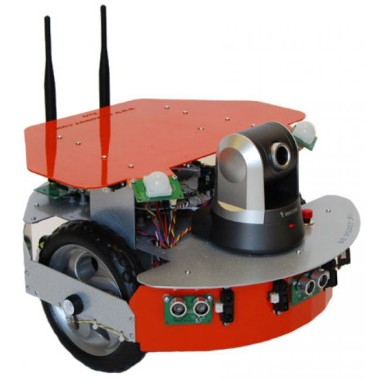
\includegraphics[width=0.3\textwidth]{figures/introduccion/robot.jpg}
		\caption{Navegación en robótica mediante \acrshort{va}}
		\label{fig.robot}
		\end{center}
\end{figure}


Otro ejemplo donde la \acrshort{va} supone un gran avance es en la comunidad médica, donde permite diagnosticar con mayor rapidez y detalle enfermedades y lesiones. De esta forma es posible aplicar tratamientos personalizados y eficaces en menor tiempo. Un claro ejemplo de investigadores que emplean \acrshort{va} es el \acrfull{csail}~\cite{cancer}, donde el desarrollo de algoritmos que analizan mamografías de una forma novedosa permite ayudar a detectar el cáncer de mama (Figura \ref{fig.cancer}) con hasta cinco años de anticipación.\\

\begin{figure}[H]
  \begin{center}
    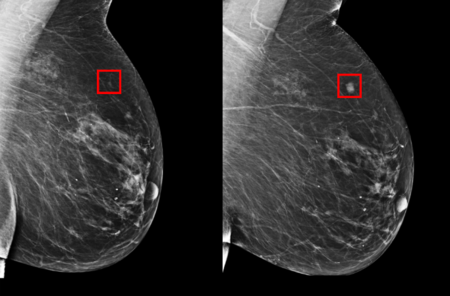
\includegraphics[width=0.4\textwidth]{figures/introduccion/cancer.png}
		\caption{Detección de cáncer de mama}
		\label{fig.cancer}
		\end{center}
\end{figure}


Una posible aplicación es el mantenimiento e inventariado urbano. Es posible identificar problemas en instalaciones y mobiliario urbano (averías, mal estado de contenedores (Figura \ref{fig.contenedor}), socavones en la vía pública, etc) mediante cámaras ubicadas por ejemplo en autobuses. Los mantenimientos de infraestructuras de transporte, como vías y cables ferroviarios, pueden programarse automáticamente implantando sistemas de \acrshort{va} en los propios trenes. 


\begin{figure}[H]
  \begin{center}
    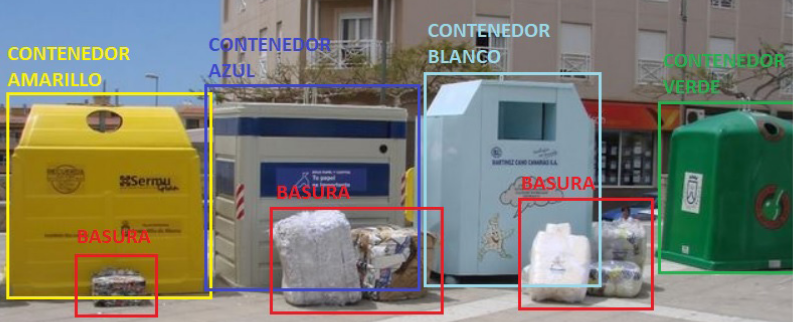
\includegraphics[width=0.5\textwidth]{figures/introduccion/contenedor.png}
		\caption{Detección de contenedores}
		\label{fig.contenedor}
		\end{center}
\end{figure}

La reducción de accidentes gracias a vehículos autónomos es una realidad gracias a la \acrshort{va}, ya que los sistemas de guiado que poseen estos vehículos están basados en esta visión. Algunos ejemplos de estos sistemas (Figura \ref{fig.car}) son: los sistemas de aviso de cambio de carril, o de control de velocidad de crucero. 

\begin{figure}[H]
  \begin{center}
    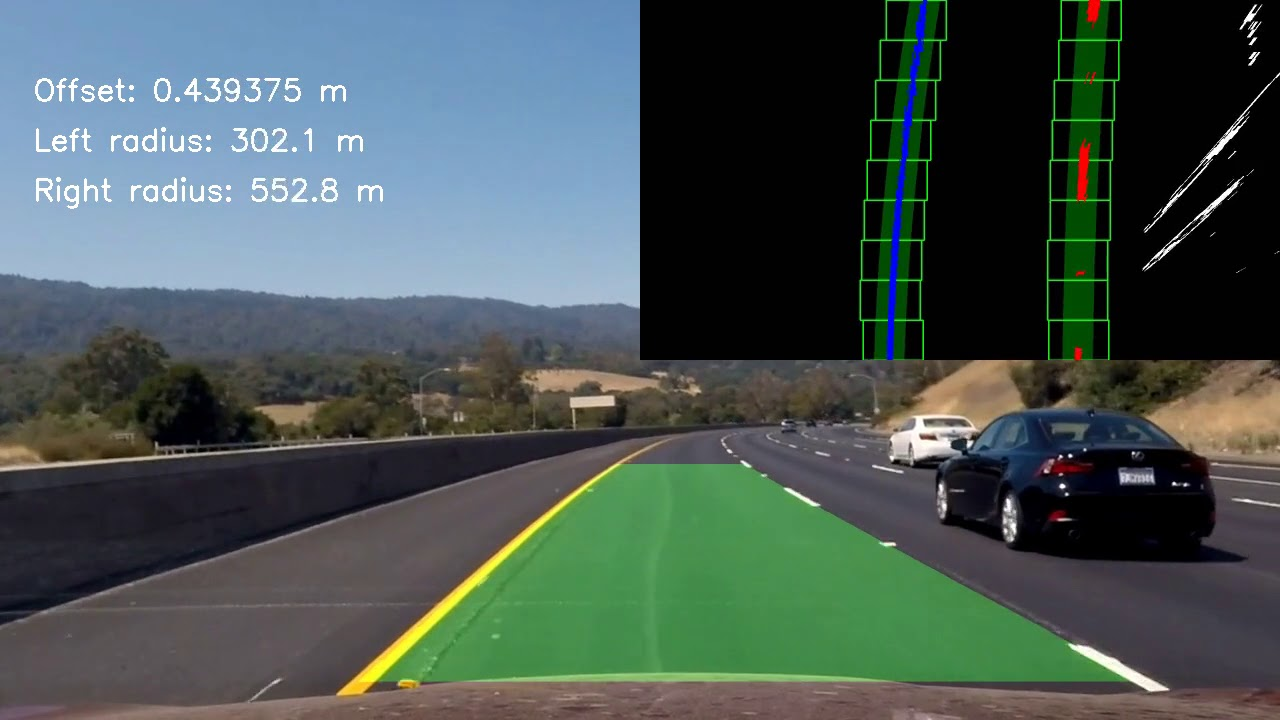
\includegraphics[width=0.5\textwidth]{figures/introduccion/car.jpg}
		\caption{Conducción autónoma}
		\label{fig.car}
		\end{center}
\end{figure}

\section{Robótica educativa}
La robótica educativa es un campo en auge debido al gran desarrollo de la robótica y la necesidad creciente de especialistas y profesionales en todo el mundo. En 2015, la Comunidad de Madrid introdujo la asignatura “Tecnología, Programación y Robótica” en el plan docente de Enseñanza Secundaria[1]. En el año 2020- 2021 se prevé implantar la asignatura “Programación y Robótica” en el plan docente de Enseñanza Primaria[2]. 

Alineado con la robótica se ha creado la educación STEM (Science, Technology, Engineering and Mathematics). Esta nueva forma de enseñanza promueve el pensamiento científico y la adquisición de conocimientos tecnológicos aplicables a situaciones reales permitiendo el desarrollo de competencias en la resolución de problemas.

Para poder impartir este tipo de asignaturas es necesaria la infraestructura adecuada. Las plataformas como la de \textit{LEGO} o la de \textit{Arduino} permiten una enseñanza y aprendizaje sencillos de la robótica resultando muy gratificante para el alumno por lo vistoso de los resultados y la obtención de una aplicación real inmediata.

\subsection{Plataformas y entornos STEM}
Es importante acercar este conocimiento tan complejo de manera adecuada a edades cada vez más tempranas para permitir un mayor desarrollo en el conocimiento de esta tecnología. Es por ello que cada vez hay más plataformas que desarrollan software orientado a niños. Algunos ejemplos de plataformas educativas son: 
\begin{itemize}
  \item Scratch\cite{Scratch}. Es un proyecto utilizado en docencia y liderado por el \textit{MIT}\footnote{\url{https://www.mit.edu}} para programar animaciones, interacciones y juegos de manera sencilla por su interfaz visual. Toda la funcionalidad de un lenguaje de programación está embebida en bloques gráficos que agrupan funcionalidades específicas.
  \item LEGO\cite{Lego}. Se trata de una plataforma que dispone de multitud de robots programables con su sistema gráfico.
  \item Kodu\cite{Kodu}. Es un sistema de programación visual para el desarrollo de videojuegos desarrollado por Microsoft\footnote{\url{https://www.microsoft.com/es-es}}
  \item Snap!\cite{Snap}. Se trata de un plataforma basada en Scratch pero con funcionalidad destinada a edades más avanzadas que permiten el desarrollo de funcionalidad más compleja.
  \item OpenRoberta\footnote{\url{https://lab.open-roberta.org/}} [7]. Es una plataforma educativa en la nube desarrollada por el instituto alemán Fraunhofer IAIS para que los niños puedan programar robots utilizando Lego Mindstorms o robots programables de LEGO (Figura \ref{fig.roberta})
  \begin{figure}[H]
  \begin{center}
    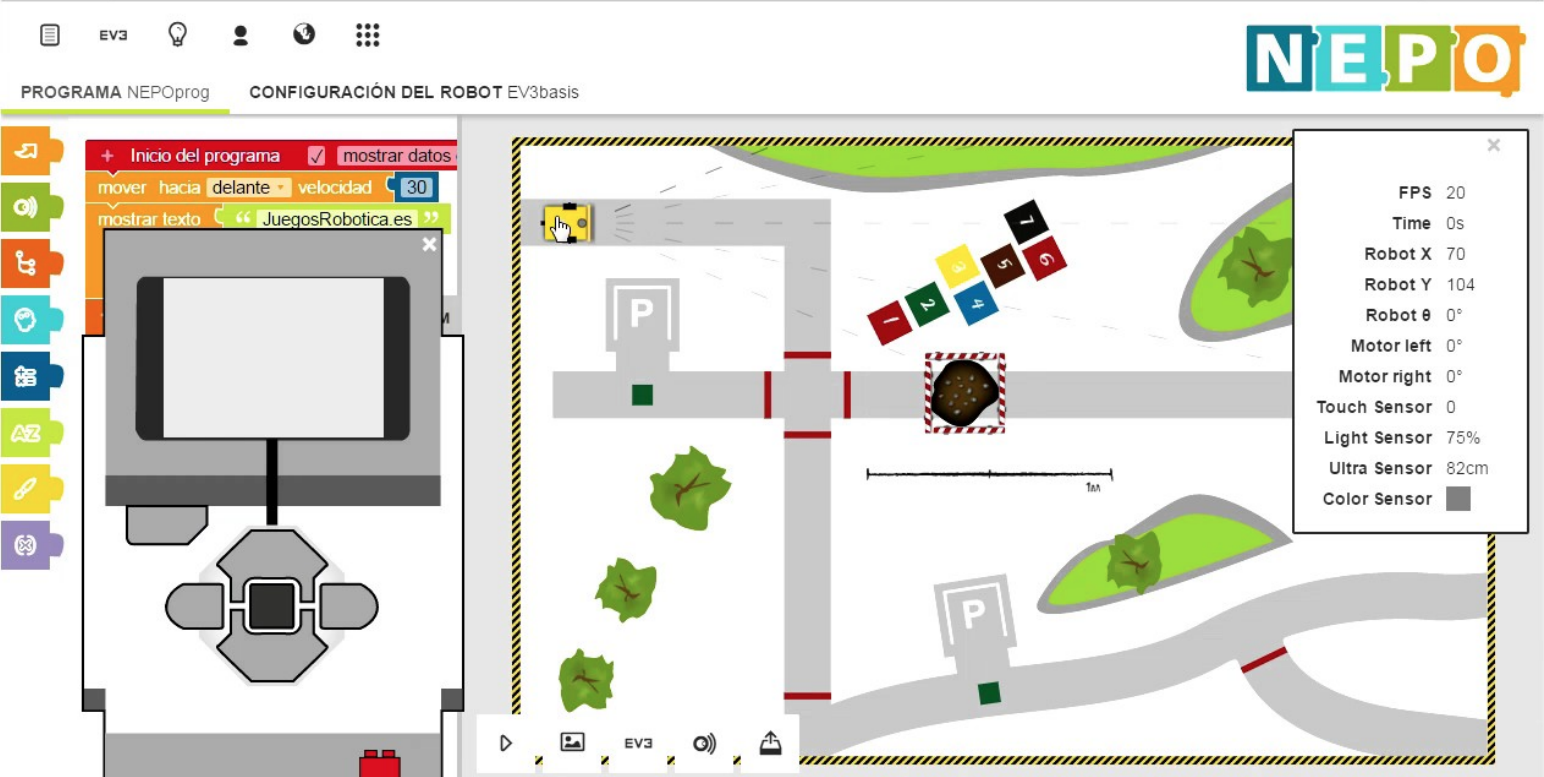
\includegraphics[width=0.5\textwidth]{figures/introduccion/openRoberta.png}
		\caption{Plataforma Open Roberta}
		\label{fig.roberta}
		\end{center}
\end{figure}
  \item Vex\footnote{\url{https://www.vexrobotics.com/}}. Plataforma orientada a la disciplina STEM de enseñanza que ofrece una gran cantidad de robots programables, así como tutoriales para aprender a montarlos y manejarlos. 
  \item AppInventor\footnote{\url{https://appinventor.mit.edu/}}. Es un entorno de desarrollo software creado por Google Labs y actualmente mantenido por el \textit{MIT} que ofrece toda la infraestructura necesaria para crear aplicaciones en Android. De esta manera, y visualmente, el usuario puede desarrollar una aplicación con bloques de código visuales, parecidos a Scratch.
  \item Arduino Web Editor\footnote{\url{https://create.arduino.cc/}}. Arduino Web Editor es una plataforma que proporciona al usuario todo lo necesario para poder programar su código en línea. De esta manera, no es necesario que el usuario instale ningún tipo de software en su sistema. Esto facilita mucho el aprendizaje dado que es inmediato (Figura \ref{fig.arduino})
  
\end{itemize}
 \begin{figure}[H]
  \begin{center}
    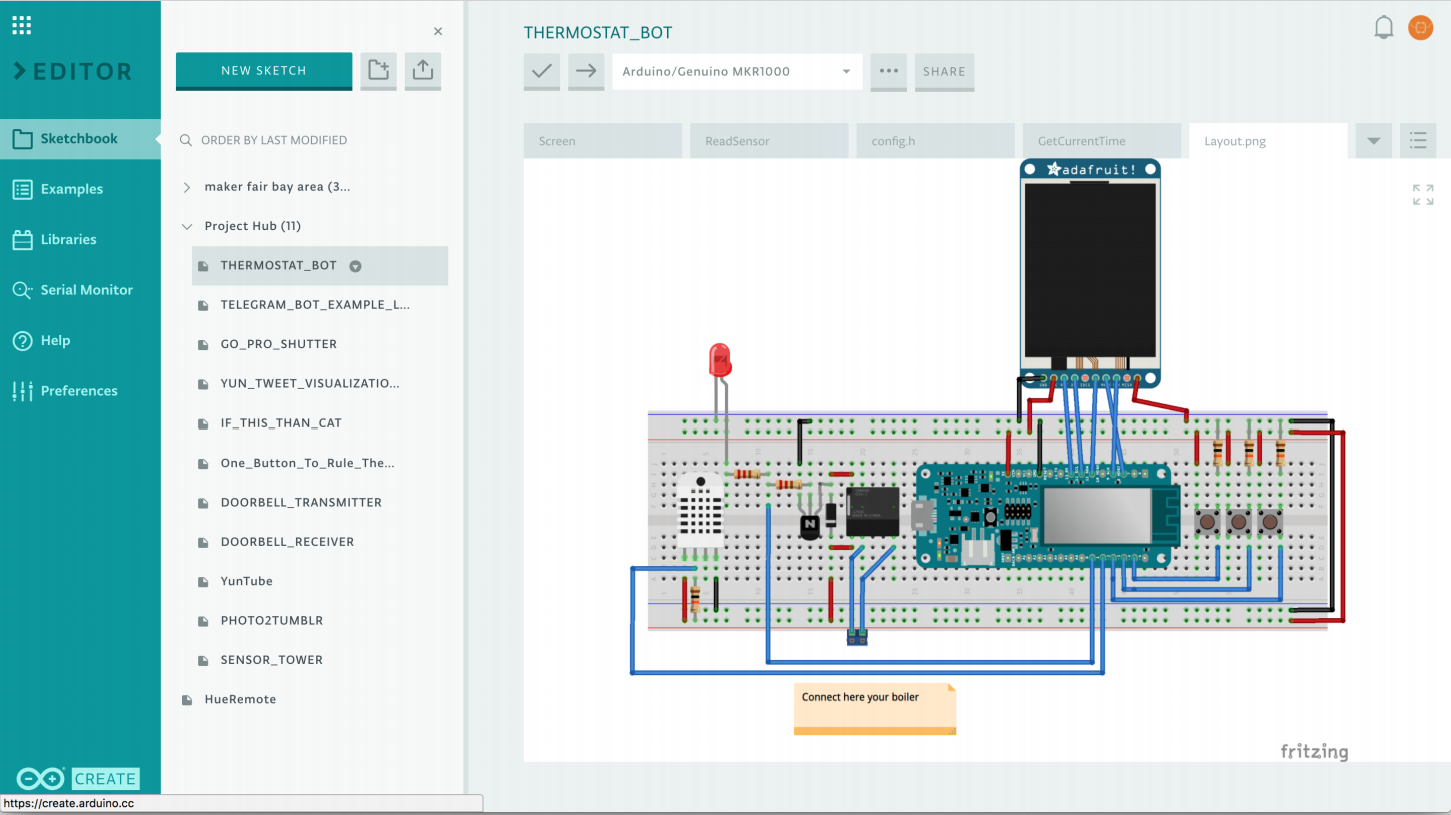
\includegraphics[width=0.5\textwidth]{figures/introduccion/arduino.png}
		\caption{\textit{Arduino} Web Editor}
		\label{fig.arduino}
		\end{center}
\end{figure}
Otra plataforma de robótica educativa, en la que se ha desarrollado este trabajo, es \textit{Kibotics} (Figuras \ref{fig:inKib1} y \ref{fig:inKib2}), que ofrece distintos entornos simulados y controlados con robots a los alumnos. Con esto, los alumnos pueden programar la inteligencia de robots autónomos para que realicen distintas pruebas sin ningún riesgo. De esta manera es posible aprender robótica en casi cualquier edad de manera sencilla y con la única necesidad de acceso a internet. Figura 1.15: Plataforma \textit{Kibotics} Figura 1.16: Página principal de \textit{Kibotics} 
\begin{figure}[!htb]
\minipage{0.45\textwidth}
    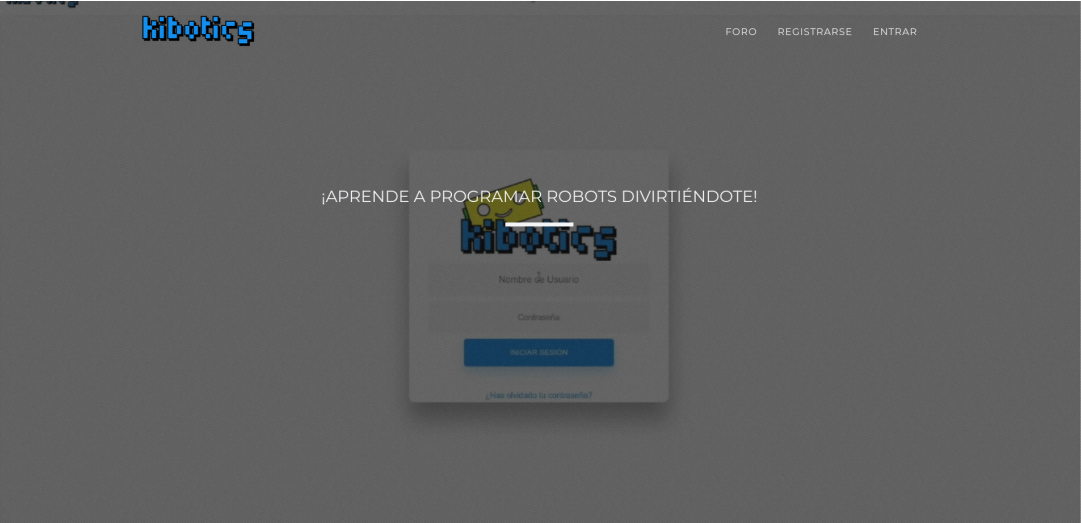
\includegraphics[width=\linewidth]{figures/introduccion/kibotics1.png}
    \caption{Plataforma \textit{Kibotics}}\label{fig:inKib1}
\endminipage\hfill
\minipage{0.45\textwidth}
    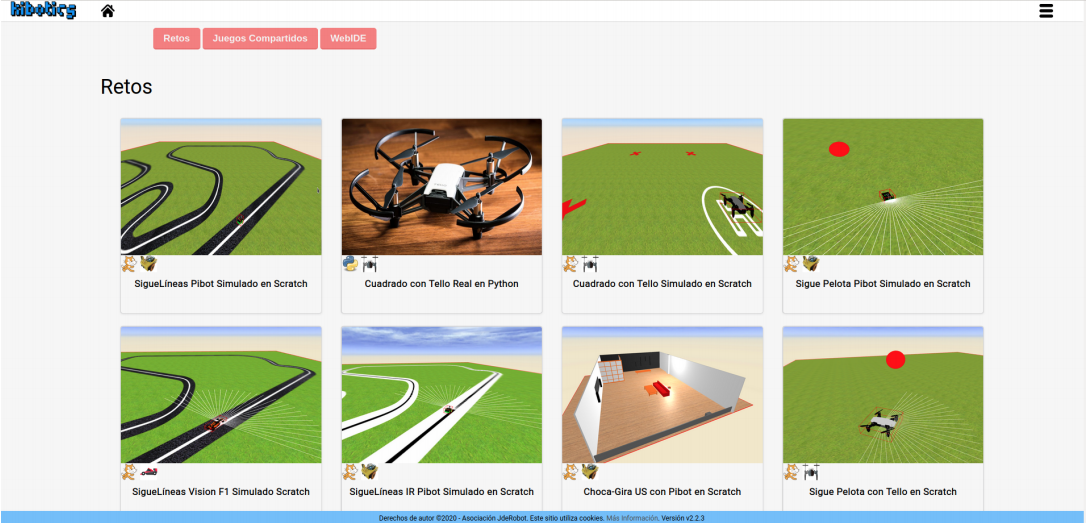
\includegraphics[width=\linewidth]{figures/introduccion/kibotics2.png}
    \caption{Página principal de \textit{Kibotics}}\label{fig:inKib2}
\endminipage\hfill
\end{figure}


Esta plataforma permite el aprendizaje de la robótica con un simulador en un entorno web. De esta manera, los usuarios sólo necesitan conexión a internet. Soporta distintos modelos de robots como el dron Tello o el Mbot, entre otros, tanto de manera simulada como en los robots reales. Además dispone de dos lenguajes de programación, Scratch(Figura \ref{fig:inKib3}) y Python (Figura \ref{fig:inKib4}) para llegar a usuarios de distintas edades.
\begin{figure}[!htb]
\minipage{0.45\textwidth}
    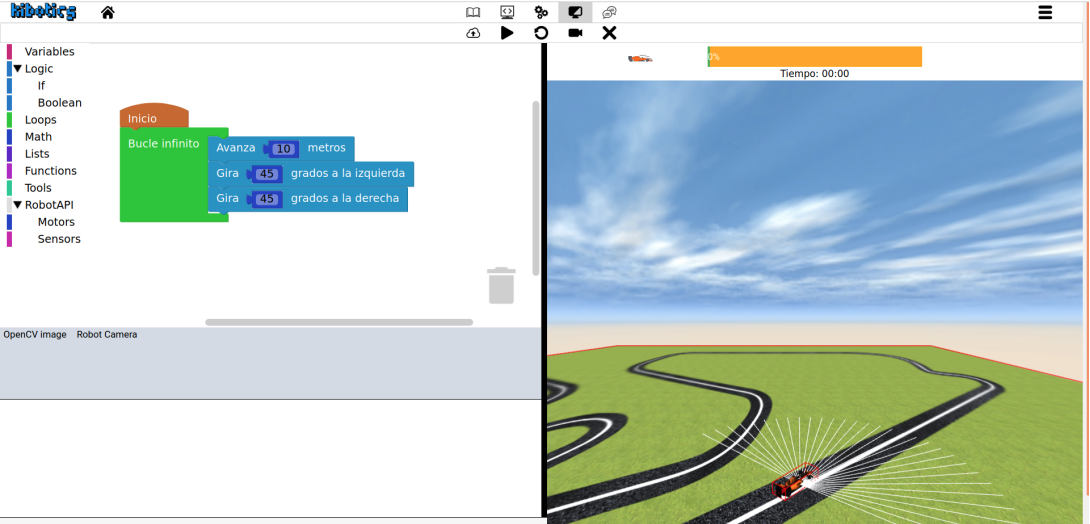
\includegraphics[width=\linewidth]{figures/introduccion/kibotics3.png}
    \caption{Editor y simulador de un ejercicio \textit{Scratch}}\label{fig:inKib3}
\endminipage\hfill
\minipage{0.45\textwidth}
    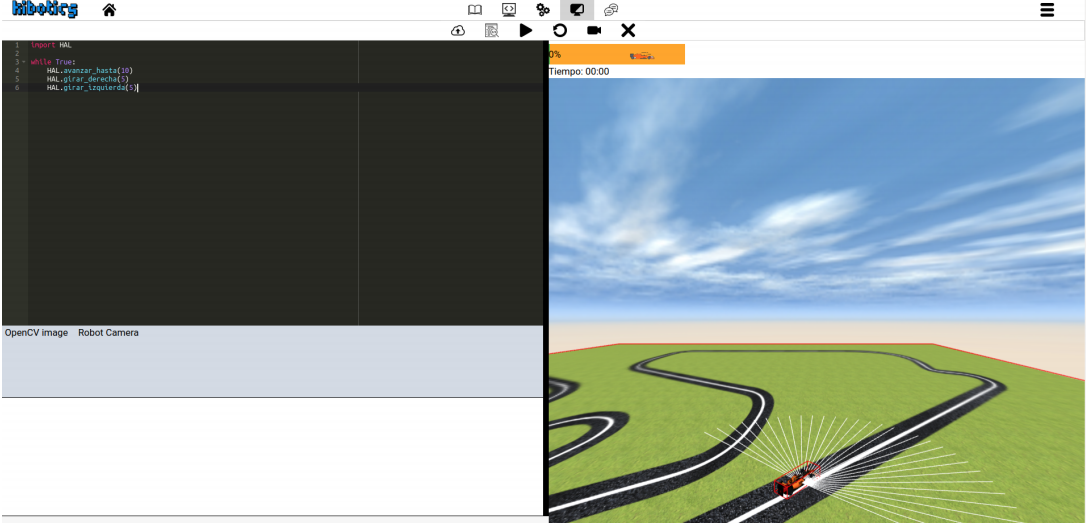
\includegraphics[width=\linewidth]{figures/introduccion/kibotics4.png}
    \caption{Editor y simulador de un ejercicio \textit{Python}}\label{fig:inKib4}
\endminipage\hfill
\end{figure}

\lhead[]{CAPÍTULO \thechapter. OBJETIVOS}
\section{Objetivos}\label{sec.objetivos}

La meta principal de este \acrshort{tfm} ha sido la creación de la arquitectura necesaria que permite añadir el uso de procesamiento visual complejo de manera sencilla en la plataforma \textit{Kibotics}. Este objetivo se ha dividido a su vez en otros dos subobjetivos.

\begin{itemize}
  \item \textbf{Comportamiento SiguePersona visual con drone real} que permite tener la infraestructura preparada para poder usarlo en los cursos que se desarrollan en la plataforma.
  \item \textbf{Comportamiento SiguePersona visual con drone simulado} para tener la infraestructura preparada también en el entorno simulado.
\end{itemize}

\subsection*{Requisitos}
Las soluciones a desarrollar para alcanzar los objetivos descritos deben cumplir además, los siguientes requisitos:

\begin{itemize}
  \item El desarrollo de la versión real debe hacerse en \textit{Python 3}.
  \item Para el desarrollo del código en la versión simulada se debe usar \textit{HTML-5}, \textit{CSS-3} y \textit{Javascript}.
  \item Debe funcionar dentro de \textit{Kibotics v2.0} o superior.
\end{itemize}
\lhead[]{CAPÍTULO \thechapter. ESTADO DEL ARTE}
\chapter{Estado del arte}\label{cap.estado}

Extado del arte
\lhead[]{CAPÍTULO \thechapter. HERRAMIENTAS}
\include{capitulos/4-Herraminetas}
\lhead[]{CAPÍTULO \thechapter. DRONE REAL}
\chapter{Comportamiento SiguePersona visual con Drone real}\label{cap.real}
En este capítulo se explica el software que se ha desarrollado para conseguir un comportamiento sigue persona con un drone real con el objetivo de ser incluido en la plataforma \textit{Kibotics} para enseñanza de robótica.

Para ello se ha tenido que perfeccionar el driver aportado por el fabricante \cite{tellodriver}. Además, como va a ser usado por niños, se ha incorporado una nueva función al interfaz sencilla de usar, por ejemplo, en vez de tener que programar la detección de un objeto de un color indicado, se ha creado un método que recibe como parámetro el nombre del color y devuelve el cuadro que rodea dicho objeto.

\section{Diseño}
La aplicación desarrollada se compone de 2 partes claras, típicas en los comportamientos robóticos sencillos: una parte perceptiva y una parte de toma de decisiones de control, ambas se ejecutan continuamente, en un bucle infinito de iteraciones (Figura \ref{fig:esquemaReal}). La primera es la detección neuronal de objeto en la imagne usando \textit{TensorFlowJS} y la segunda son tres controladores PID que gobiernan el movimiento del drone en tres ejes, el delante-detrás, el arriba-abajo y el giro izquierda-derecha..
\begin{figure}[H]
  \begin{center}
    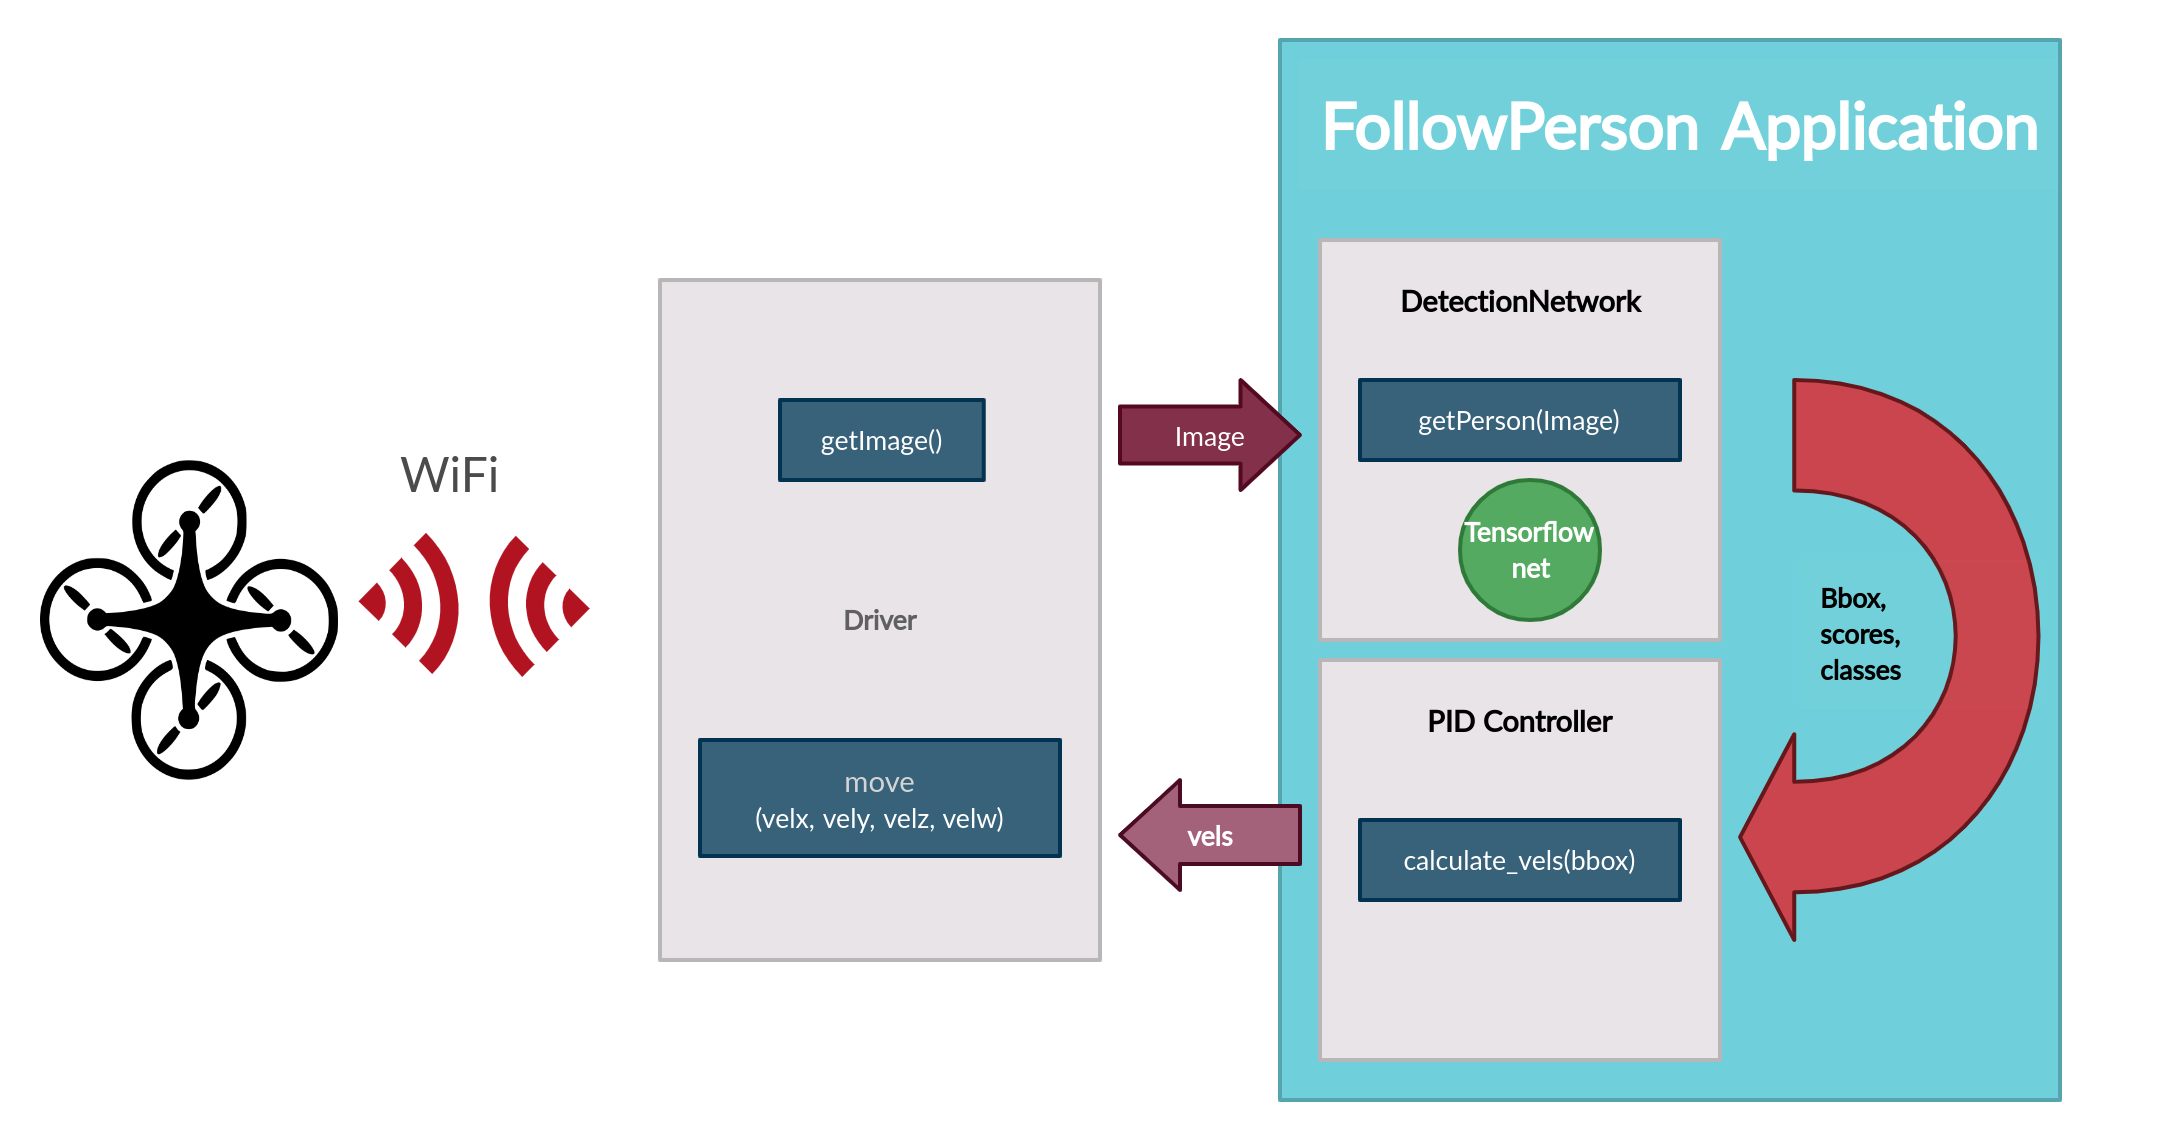
\includegraphics[width=0.9\textwidth]{figures/real/esquema2.png}
		\caption{Diseño de la aplicación SiguePersona visual}
		\label{fig:esquemaReal}
		\end{center}
\end{figure}

La detección neuronal es un recubrimiento de la red neuronal que recibe las imágenes del driver y devuelve los \textit{bounding boxes}, puntuaciones y clases detectadas. 
La parte de los controladores usando los \textit{bounding boxes} calcula la velocidades y se las pasa al driver.


\section{Desarrollo del \textit{driver} real}
El \textit{driver} desarrollado para la plataforma \textit{Kibotics} parte del proporcionado por el fabricante del drone. Se han añadido una serie de cambios por las limitaciones detectadas, además de necesitar simplificar el uso ya que está orientado a enseñanza infantil. 

Este \textit{driver} permite recibir imágenes de la cámara del drone, recibir informaciones básicas como batería restante o tiempo de vuelo. Además permite controlar el drone tanto en velocidad como en posición (avanza x metros, gira x grados,...), ...\\

El driver ejecuta en el ordenador, que a su vez está en continua comunicación con el drone \textit{Tello} a través de la red \textit{WiFi} que levanta de modo automático el propio drone. El driver no ejecuta a bordo del cuadricóptero.

\subsection{Primera versión}
Esta primera versión tiene el objetivo de subsanar los siguientes problemas:
\begin{itemize}
  \item El \textit{driver} no tiene control en velocidad, , sólo control en posición, que se consigue gracias a la cámara ventral y la estabilización visual que proporciona el fabricante, como mecanismo de seguridad.
  \item Si pasan 5 segundos sin recibir mensajes el drone se desactiva
  \item Las velocidades de entrada están en \textbf{cm/s} y \textbf{grados/s} de las funciones del driver del fabricante.
\end{itemize}

\subsubsection*{No tiene control en velocidad}
El \textit{driver} aportado por el fabricante en \textit{Python} viene sin control en velocidad. Sí trae opciones para poder dar valor a las velocidades usadas por el drone y control en posición, pero no control en velocidad.
Después de analizar el documento del \acrshort{sdk}\footnote{\url{https://terra-1-g.djicdn.com/2d4dce68897a46b19fc717f3576b7c6a/Tello\%20\%E7\%BC\%96\%E7\%A8\%8B\%E7\%9B\%B8\%E5\%85\%B3/For\%20Tello/Tello\%20SDK\%20Documentation\%20EN_1.3_1122.pdf}} se vio que sí existe un comando planeado para el control en velocidad, pero que no se ha implementado realmente en el \textit{driver} aportado. 
Se implementa dicho método en el \textit{driver} desarrollado. Además, se implementa un hilo que se encarga de enviar cada poco tiempo la velocidad (500ms) como recordatorio porque, si no, como mecanismo de seguridad el drone se detiene si no recibe más mensajes de velocidad.

\subsubsection*{Las velocidades de entrada están en \textbf{cm/s} y \textbf{grados/s}}
La intención ha sido que se use el Sistema Internacional en todo momento y en este caso son \textbf{m/s} y \textbf{rad/s}.
Esto es tan fácil como realizar las conversiones pertinentes en las funciones para establecer las velocidades.

\subsubsection*{Si pasan 5 segundos sin recibir mensajes el drone se desactiva}
Este problema ha sido resuelto añadiendo un hilo de \textbf{Python} (perro de guarda, \textit{watchdog}) que se encarga de enviar velocidades cada \textbf{500ms}. De esta manera evitamos que el \textit{Drone} se desactive.

\subsection{Segunda versión}
Los problemas subsanados en esta versión han sido los siguientes:
\begin{itemize}
  \item \textit{Driver} es necesario en Python 3.x pero en la primera versión está escrito en Python 2.7. 
  \item Poca fiabilidad en el envío de mensajes del \textit{driver} al drone.
  \item El control en velocidad es poco reactivo.
\end{itemize}
\subsubsection*{Convertir el \textbf{driver} de Python 2.7 a Python 3.x}
Esto ha sido fácil porque casi todo el código de la aplicación funcionaba en Python 3, las únicas diferencias eran la manera de importar los módulos que varía de entre las dos versiones y que en Python 2 los bytes se representan como cadenas de texto(\textit{String}) y en Python 3 son del tipo bytes.
\begin{table}[H]
\centering
\begin{tabular}{|c|c|c|}
\hline
\textbf{Tipo de cambio}          & \textbf{Python 2} & \textbf{Python 3} \\ \hline
Representación de bytes          & ' '               & b' '              \\ \hline
Importar desde mismo repositorio & import module     & import .module    \\ \hline
\end{tabular}
\caption{Cambios de Python 2 a Python 3 efectuados}
\label{tab:cambios_python_2_3}
\end{table}

En la tabla \ref{tab:cambios_python_2_3} se pueden ver los cambios efectuados.

\subsubsection*{Poca fiabilidad en el envío de mensajes del \textit{driver} al drone}
La comunicación con el Drone consiste en enviar un mensaje y recibir una respuesta que confirma que lo ha recibido, o en el caso de pedirle algún dato como la batería restante el dato en si.

El problema radica en que frecuentemente en la \textit{WiFi} que comunica drone y ordenador o se pierde el mensaje que se envía o  se pierde la respuesta. Por lo que se ha implementado un mecanismo de reenvío de mensajes. Si no se recibe respuesta se vuelve a enviar el mismo mensaje hasta tener respuesta o se alcance el número máximo de reintentos.

\subsubsection*{El control en velocidad es poco reactivo}
 Para mejorar este apartado solo ha hecho falta reducir el tiempo entre mensajes de velocidad a \textbf{25ms}. Además, no importa que se pierdan mensajes porque enseguida se envía otro con la velocidad actualizada.

\section{Detección visual de la persona}
Para elegir la red se han comparado tres del conjunto de redes preentrenadas con el \textit{dataset} \acrshort{coco} de \textit{Object Detection API}\footnote{\url{https://github.com/tensorflow/models/blob/master/research/object_detection/g3doc/tf2_detection_zoo.md}}:
\begin{itemize}
  \item SSD Mobilenet v2 FPN de 320x320
  \item CenterNet resnet50 FPN de 512x512
  \item SSD Resnet50 FPN de 640x640
\end{itemize}
Para esta elección se ha grabado un vídeo con la cámara del drone real (720x960 píxeles), donde en todo momento hay una persona y se ha usado el mismo vídeo con las tres opciones, y en un ordenador con un procesador I7 de octava generación, 16 GB de RAM y con gráfica integrada. obteniendo los resultado de la tabla \ref{tab:comparativa_redes}.
\begin{table}[H]
\centering
\begin{tabular}{|c|c|c|c|}
\hline
\textbf{Red}          & \textbf{Tiempo} & \textbf{Detecciones} & \textbf{Score} \\ \hline 
SSD Mobilenet v2      & 90ms            & 79\%        & 64\%           \\ \hline  
SSD Resnet50 v1       & 240ms           & 86\%        & 71\%           \\\hline  
CenterNet Resnet50 v1 & 450ms           & 85\%        & 71\%           \\ \hline 
\end{tabular}
\caption{Comparativa de redes}
\label{tab:comparativa_redes}
\end{table}
Se ha elegido \textit{SSD Mobilenet v2 FPN} (Figura \ref{fig:mobilenet}) porque es la única que funciona a una velocidad razonable para incorporar un comportamiento robótico reactivo.
\begin{figure}[H]
  \begin{center}
    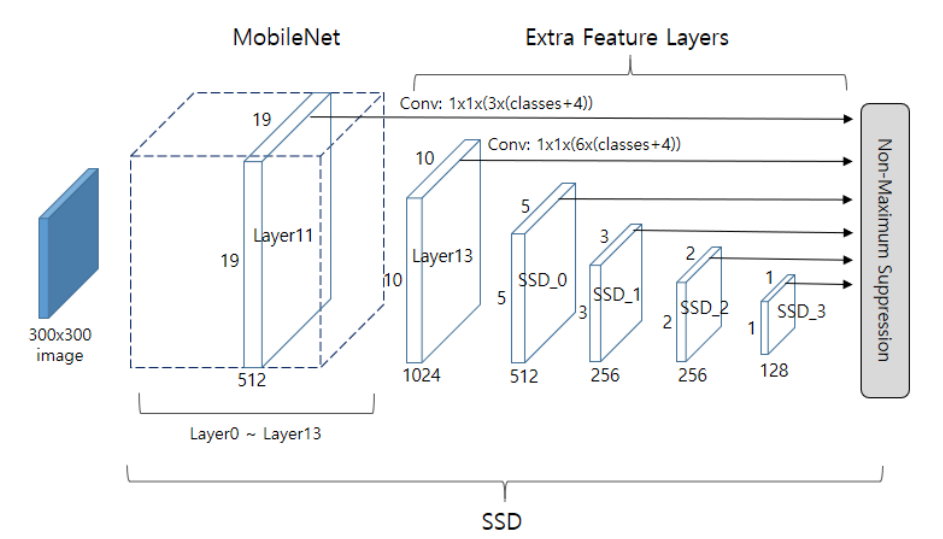
\includegraphics[width=0.8\textwidth]{figures/real/mobilenet.png}
		\caption{Esquema de una red Mobilenet \acrshort{ssd}}
		\label{fig:mobilenet}
		\end{center}
\end{figure}
Esta red tiene 2 componentes principales: 
\begin{itemize}
  \item \textit{\gls{fpn} lite}\cite{fpn}. Permite extraer características de la imagen con indiferencia del tamaño del objeto 
  \item \textit{\gls{ssd} Mobilenet v2}. Una red \acrfull{ssd} con una red base \textit{Mobilenet v2}\cite{mobilenetv2}
\end{itemize}

Para poder trabajar con ella se usa en \textit{Tensorflow 2.0}. Además se ha tenido que desarrollar un recubrimiento para poder usar la red de manera fácil.
Esta clase desarrollada permite cargar la red indicada por configuración ya sea un modelo de \textbf{Tensoflow} o un grafo. Además agrega un postprocesado de la información de salida de la red (figura \ref{fig:getPerson}): 
\begin{figure}[H]
  \begin{center}
    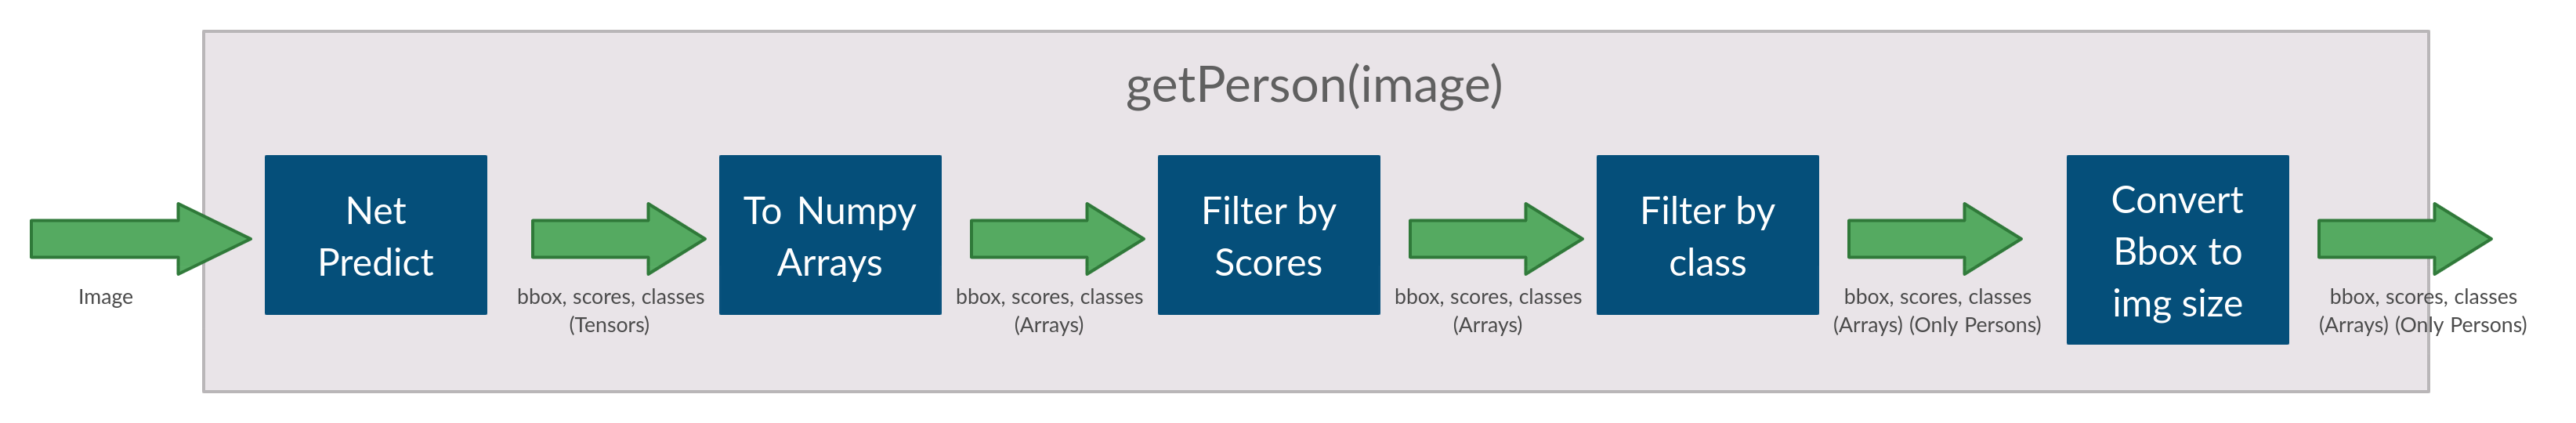
\includegraphics[width=1\textwidth]{figures/real/getPerson.png}
		\caption{Función \textit{getPerson}}
		\label{fig:getPerson}
		\end{center}
\end{figure}
\begin{itemize}
  \item convirtiendo en \textit{numpy arrays} los datos desde tensores
  \item Desechando los resultados con una puntuación menor al límite indicado por configuración.
  \item Filtrando los resultados para quedarse con las clases buscadas, en este caso personas.
  \item También se convierten los tamaños de las regiones de interés de porcentaje a píxeles.
\end{itemize}

Además, se ha creado también otro nivel de abstracción superior para la fuente de la imagen para ayudar a su uso. Así mediante configuración se indica si la fuente es el drone, una webcam, un directorio de imágenes o un vídeo y la fuente en sí y no hay que preocuparse de procesar la imagen para convertirla en RGB en caso de que sea la fuente no lo sea por ejemplo.

La red al final devuelve 3 \textit{arrays}, el primero con la clase a la que pertenecen las detecciones, el segundo con las regiones de interés o \textit{bounding boxes} (x mínima, y mínima, x máxima, y máxima) y el tercero con las puntuaciones, que indica la fiabilidad estimada de cada una de las detecciones.

Todo este procesamiento visual se ha incluido en el \textit{driver}, mediante una función llamada \textit{getPerson()}, para que pueda ser usado de manera sencilla desde las nuevas aplicaciones de robótica de los usuarios de \textit{Kibotics}, quedando integrada en dicha plataforma.

\section{Control PID}
El control PID es un bucle de control que calcula la siguiente orden a comandar al drone real en cada iteración.
\[ u(t) = K_p e(t) + K_i \int_{t}^{0} e(t') dt' + K_d \frac{de(t)}{dt}\]
Donde \textbf{e} es el error con respecto al objetivo y las  constantes $K_p$ , $K_i$ y $K_d$ que deben calcularse experimentalmente. los objetivos son centrar en la imagen la persona horizontalmente, verticalmente y con un tamaño concreto, lo que conlleva que el drone está mirando directamente a la persona a una distancia razonable.

Una vez que se procesa la imagen recibida por el drone y se tienen las detecciones, se selecciona la persona con mayor puntuación y de su \textit{bounding box} se extrae posición central, el área y la posición superior.

\begin{figure}[H]
  \begin{center}
    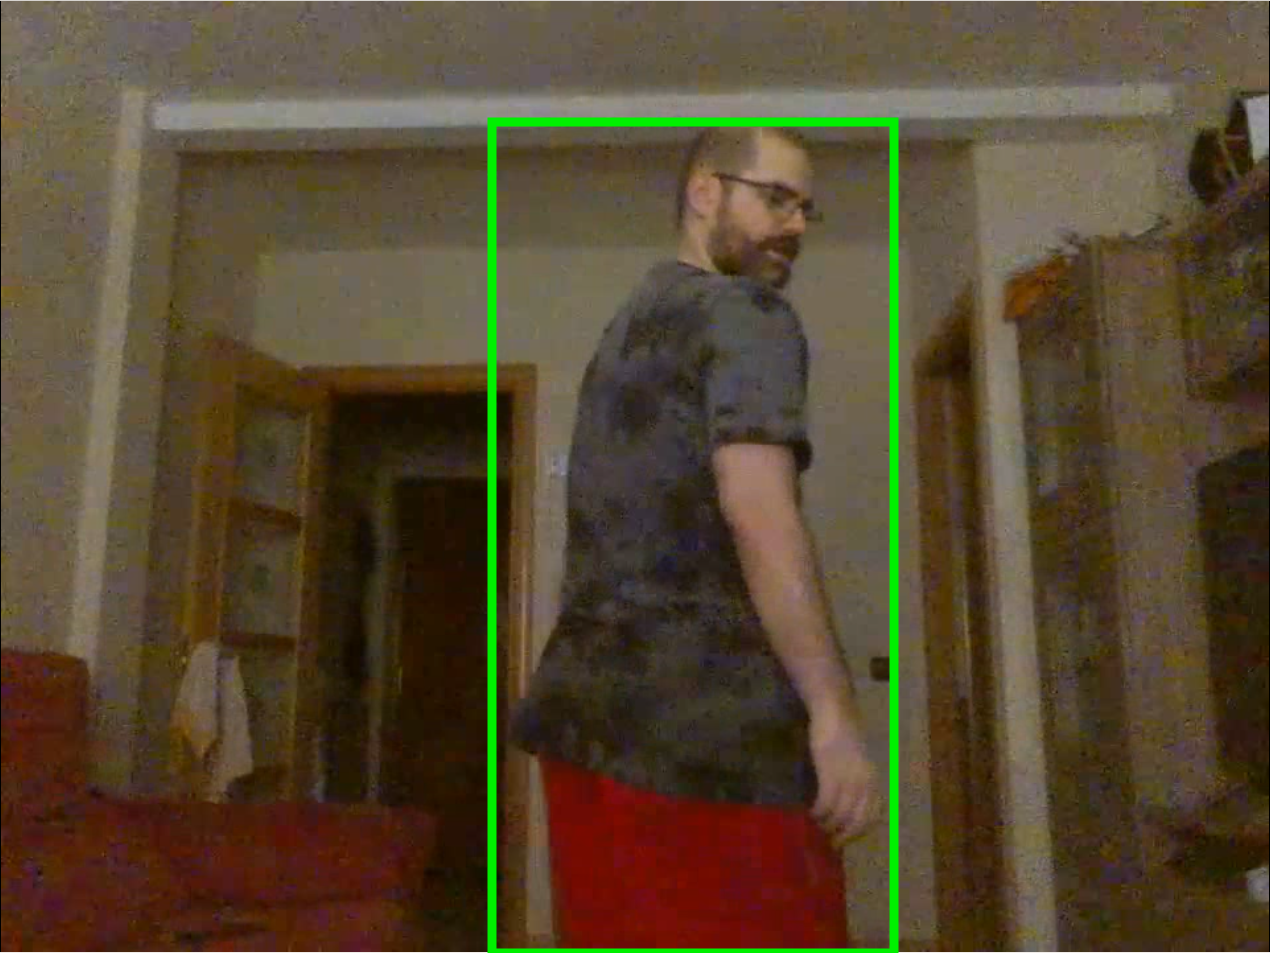
\includegraphics[width=0.6\textwidth]{figures/real/cap3.png}
		\caption{Detección de persona}
		\label{fig:bbox_ideal}
		\end{center}
\end{figure}

Para controlar el drone se va a hacer con tres velocidades, avance, giro horizontal y movimiento vertical. Para ello se utiliza un control PID (en este caso debido al funcionamiento del drone solo proporcional y derivativo) para cada una de las velocidades.
\subsection*{Control de avance}

En el caso de la velocidad de avance, se toma como referencia el área. Se fija un área objetivo para el \textit{bounding box}, si la obtenida es menor, se avanza y si es mayor se retrocede. Las constantes \textbf{proporcional y derivativa} en este caso son \textbf{0.01 y 0} respectivamente.

\subsection*{Control de giro horizontal o guiñada}

En este caso se toma como referencia la coordenada x del centro de la imagen. Si el \textit{bounding box} se mueve a la izquierda hay que girar a la izquierda y si se va a derecha igual. Las constantes, ajustadas experimentalmente, \textbf{proporcional y derivativa} en este caso son \textbf{0.7 y 0.001} respectivamente.

\subsection*{Control de elevación}
En el caso de la velocidad vertical se ha decidido usar como referencia la posición superior del \textit{bounding box} posicionándolo en torno a un 10\% de la parte superior de la imagen con el objetivo que se vea la cara de la persona. Se probó también la manera fácil, que es centrar verticalmente la persona en la imagen, pero puede ocurrir que solo se tenga una parte de la persona  en la imagen y esté centrado, como se puede ver en las imágenes \ref{fig:real1} y \ref{fig:real2}. En ambos casos el centro del rectángulo está muy próximo al centro vertical de la imagen, pero no por ello está bien.

\begin{figure}[!htb]
\minipage{0.45\textwidth}
    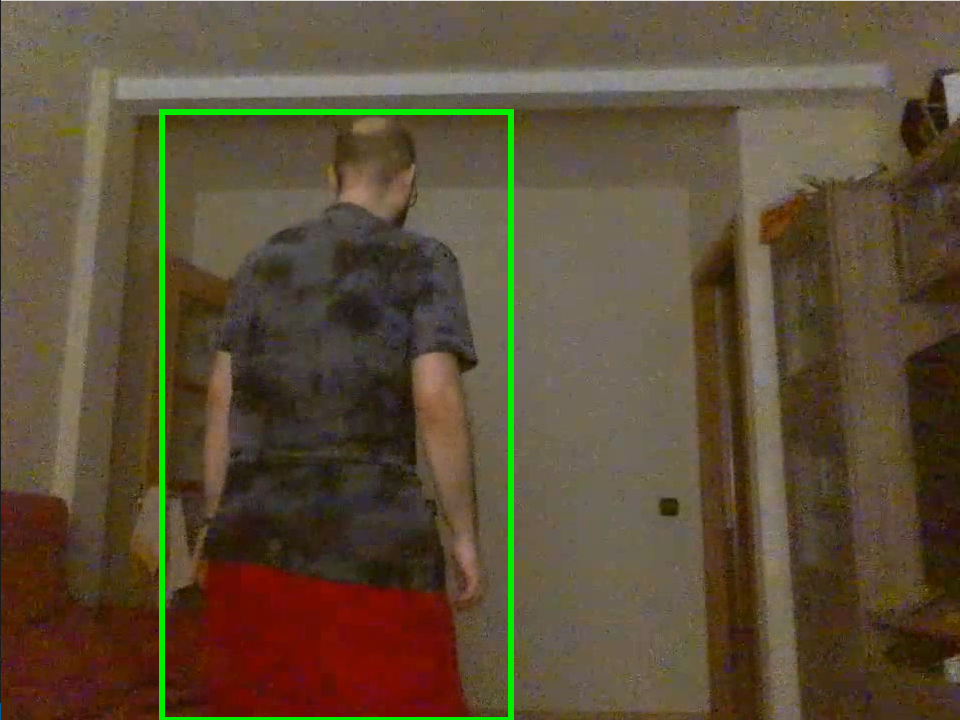
\includegraphics[width=\linewidth]{figures/real/cap1.png}
    \caption{Persona seleccionada}\label{fig:real1}
\endminipage\hfill
\minipage{0.45\textwidth}
    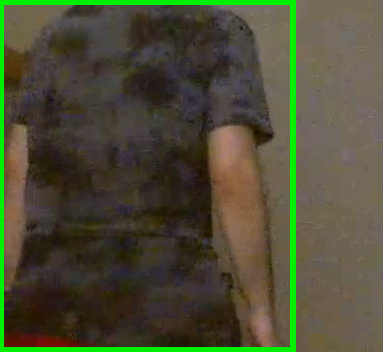
\includegraphics[width=\linewidth]{figures/real/cap2.png}
    \caption{Torso detectado}\label{fig:real2}
\endminipage\hfill
\end{figure}

En cambio tomando como referencia el punto más alto del cuadrado se tiende a obtener la imagen \ref{fig:real1}, lo que además facilita la detección de la persona.
Las constantes \textbf{proporcional y derivativa} en este caso son \textbf{3 y 0.5} respectivamente ajustadas de modo experimental. Hay que destacar además que en el caso de tener error por estar muy cerca del borde superior de la imagen se ha sumado 0.3 a dicho error para evitar que considere el borde  superior de la imagen como valor aceptable. 


\section{Validación experimental}
La validación experimental del desarrollo del software realizado se ha hecho en 4 casos, tres tests unitarios, uno por cada \textit{PID} y un test global con los tres controladores integrados y funcionando en conjunto. En todos los casos el bucle de control funciona a 7 \acrshort{fps}.

\subsection{Control de giro horizontal}
Esta prueba consiste en moverse de izquierda a derecha delante del drone para ajustar las constantes del \textit{PID} de giro horizontal (Figura \ref{fig:real_giro}).

\begin{figure}[!htb]
\minipage{0.3\textwidth}
    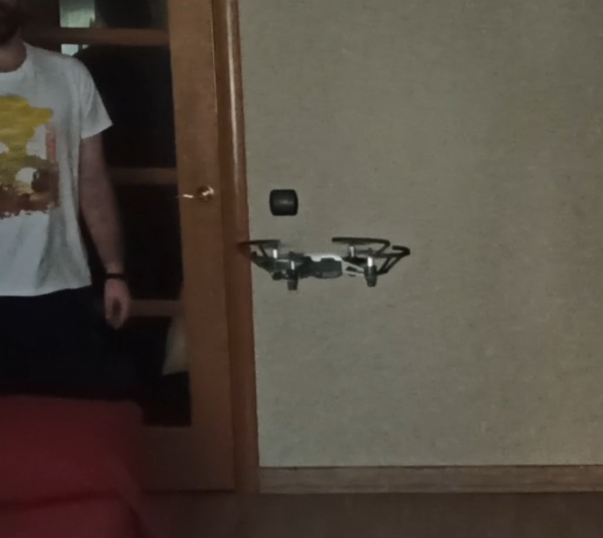
\includegraphics[width=\linewidth]{figures/real/giroR_1.png}
\endminipage\hfill
\minipage{0.3\textwidth}
    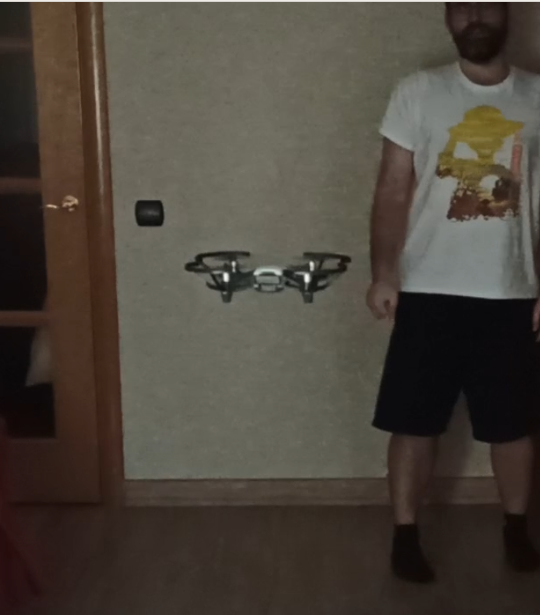
\includegraphics[width=\linewidth]{figures/real/giroR_2.png}
\endminipage\hfill
\minipage{0.3\textwidth}
    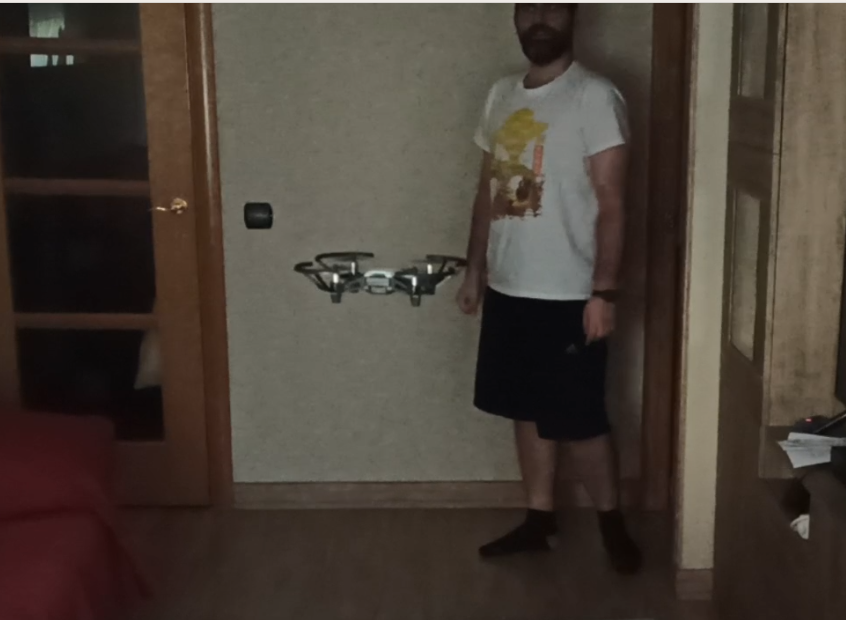
\includegraphics[width=\linewidth]{figures/real/giroR_3.png}
\endminipage\hfill
\caption{Ejemplo de giro horizontal en drone real}
\label{fig:real_giro}
\end{figure}
\subsection{Control de elevación}
Esta prueba consiste en agacharse y levantarse delante del drone para ajustar las constantes del \textit{PID} de elevación (Figura \ref{fig:real_elev}).

\begin{figure}[!htb]
\minipage{0.3\textwidth}
    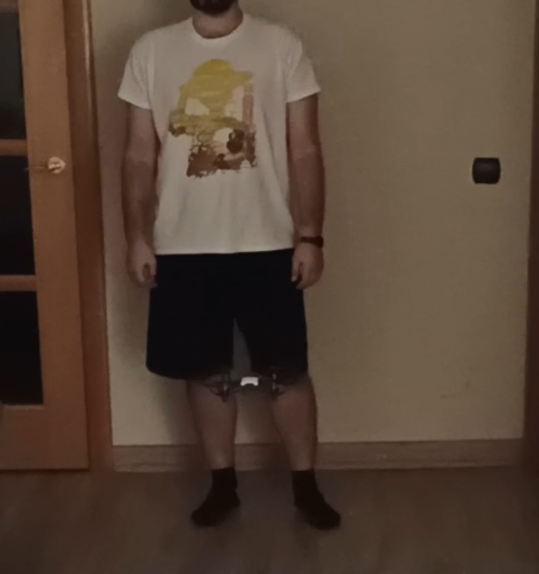
\includegraphics[width=\linewidth]{figures/real/elevacion_1.png}
\endminipage\hfill
\minipage{0.3\textwidth}
    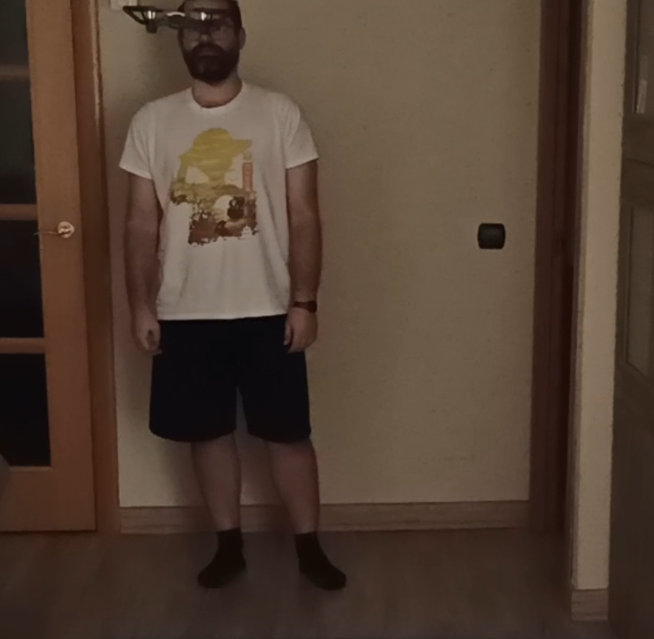
\includegraphics[width=\linewidth]{figures/real/elevacion_2.png}
\endminipage\hfill
\minipage{0.3\textwidth}
    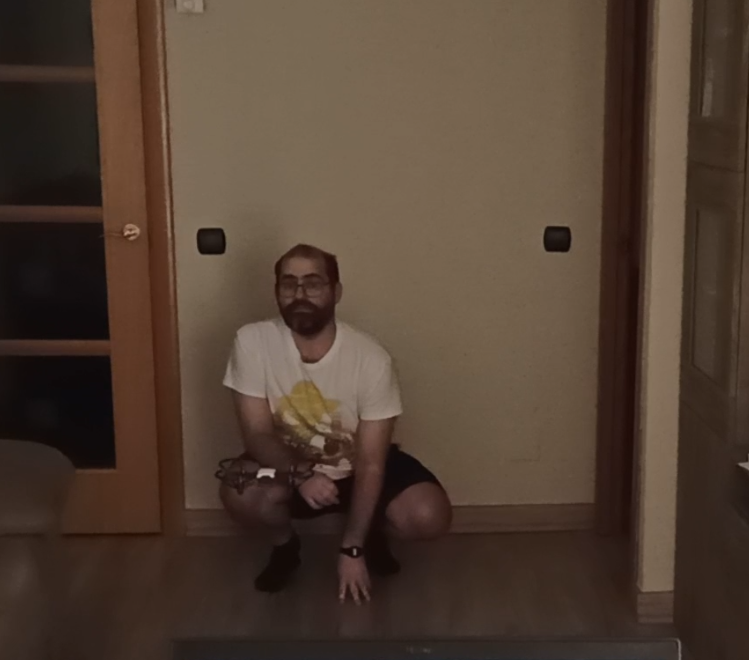
\includegraphics[width=\linewidth]{figures/real/elevacion_3.png}
\endminipage\hfill
\caption{Ejemplo de control de elevación en drone real}
\label{fig:real_elev}
\end{figure}
\subsection{Control de avance}
Esta prueba consiste en avanzar y retroceder delante del drone para ajustar las constantes del \textit{PID} de avance (Figura \ref{fig:real_avance}).

\begin{figure}[!htb]
\minipage{0.3\textwidth}
    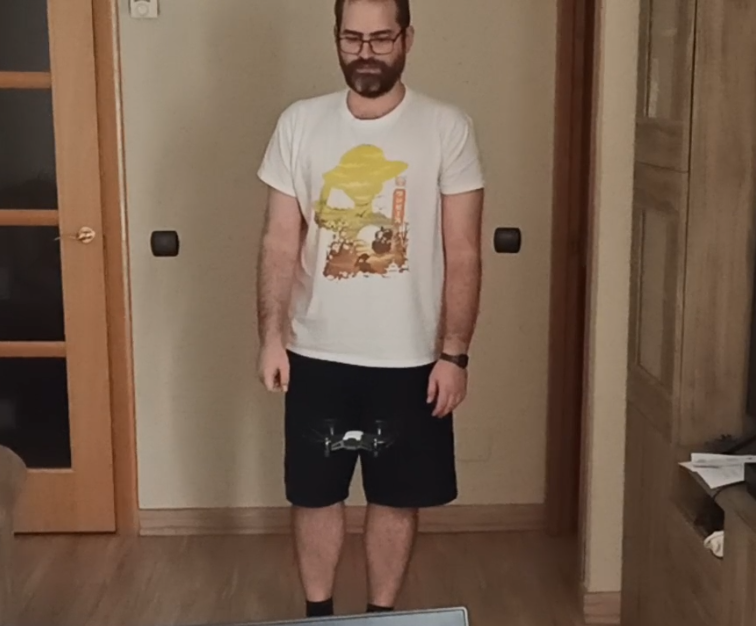
\includegraphics[width=\linewidth]{figures/real/avanceR_1.png}
\endminipage\hfill
\minipage{0.3\textwidth}
    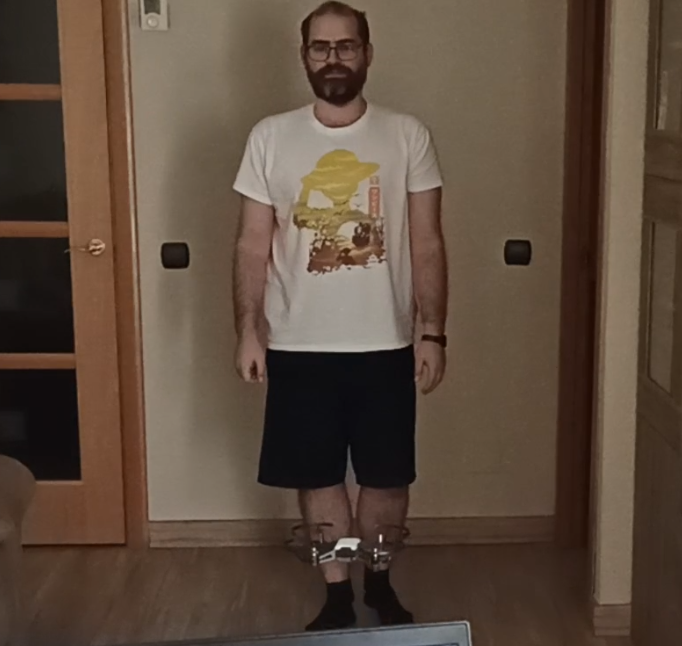
\includegraphics[width=\linewidth]{figures/real/avanceR_2.png}
\endminipage\hfill
\minipage{0.3\textwidth}
    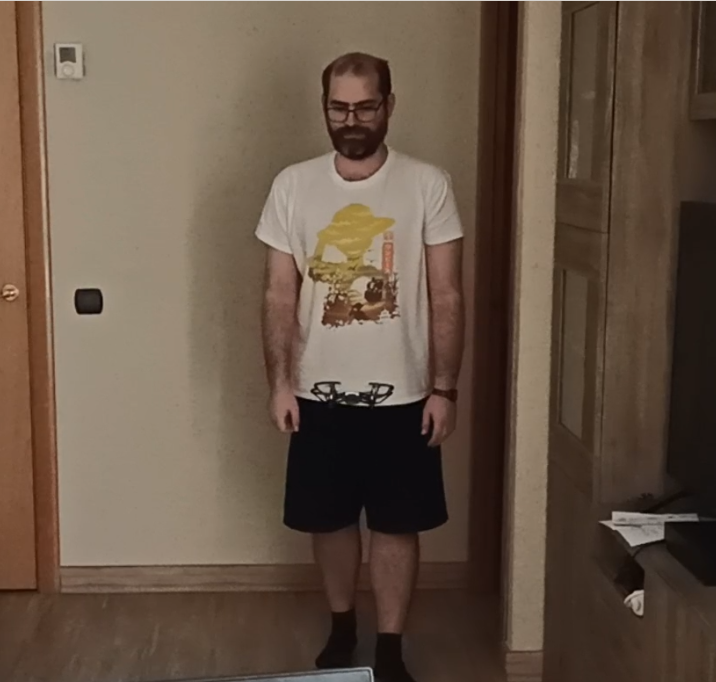
\includegraphics[width=\linewidth]{figures/real/avanceR_3.png}
\endminipage\hfill
\caption{Ejemplo de avance en drone real}
\label{fig:real_avance}
\end{figure}
\subsection{Ejecución típica completa}
Esta prueba consiste en moverse por la habitación para comprobar si el comportamiento conjunto es el correcto (Figura \ref{fig:real_com}). De no serlo, toca ajustar las constantes oportunas.

\begin{figure}[!htb]
\minipage{0.45\textwidth}
    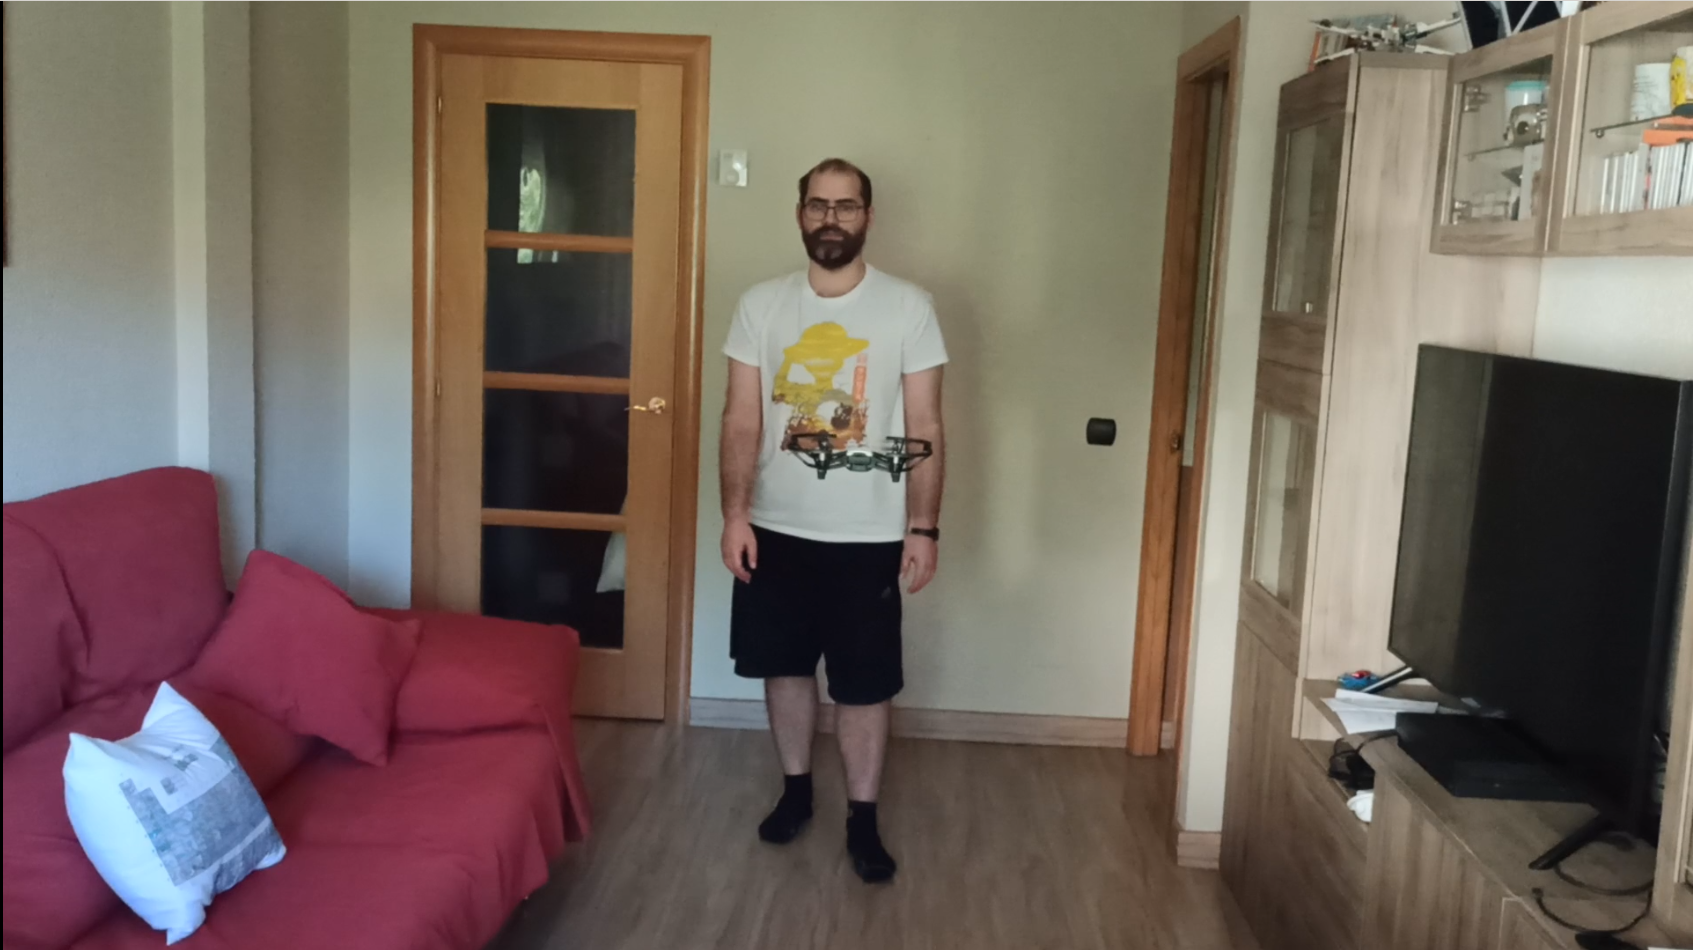
\includegraphics[width=\linewidth]{figures/real/comR_1.png}
\endminipage\hfill
\minipage{0.45\textwidth}
    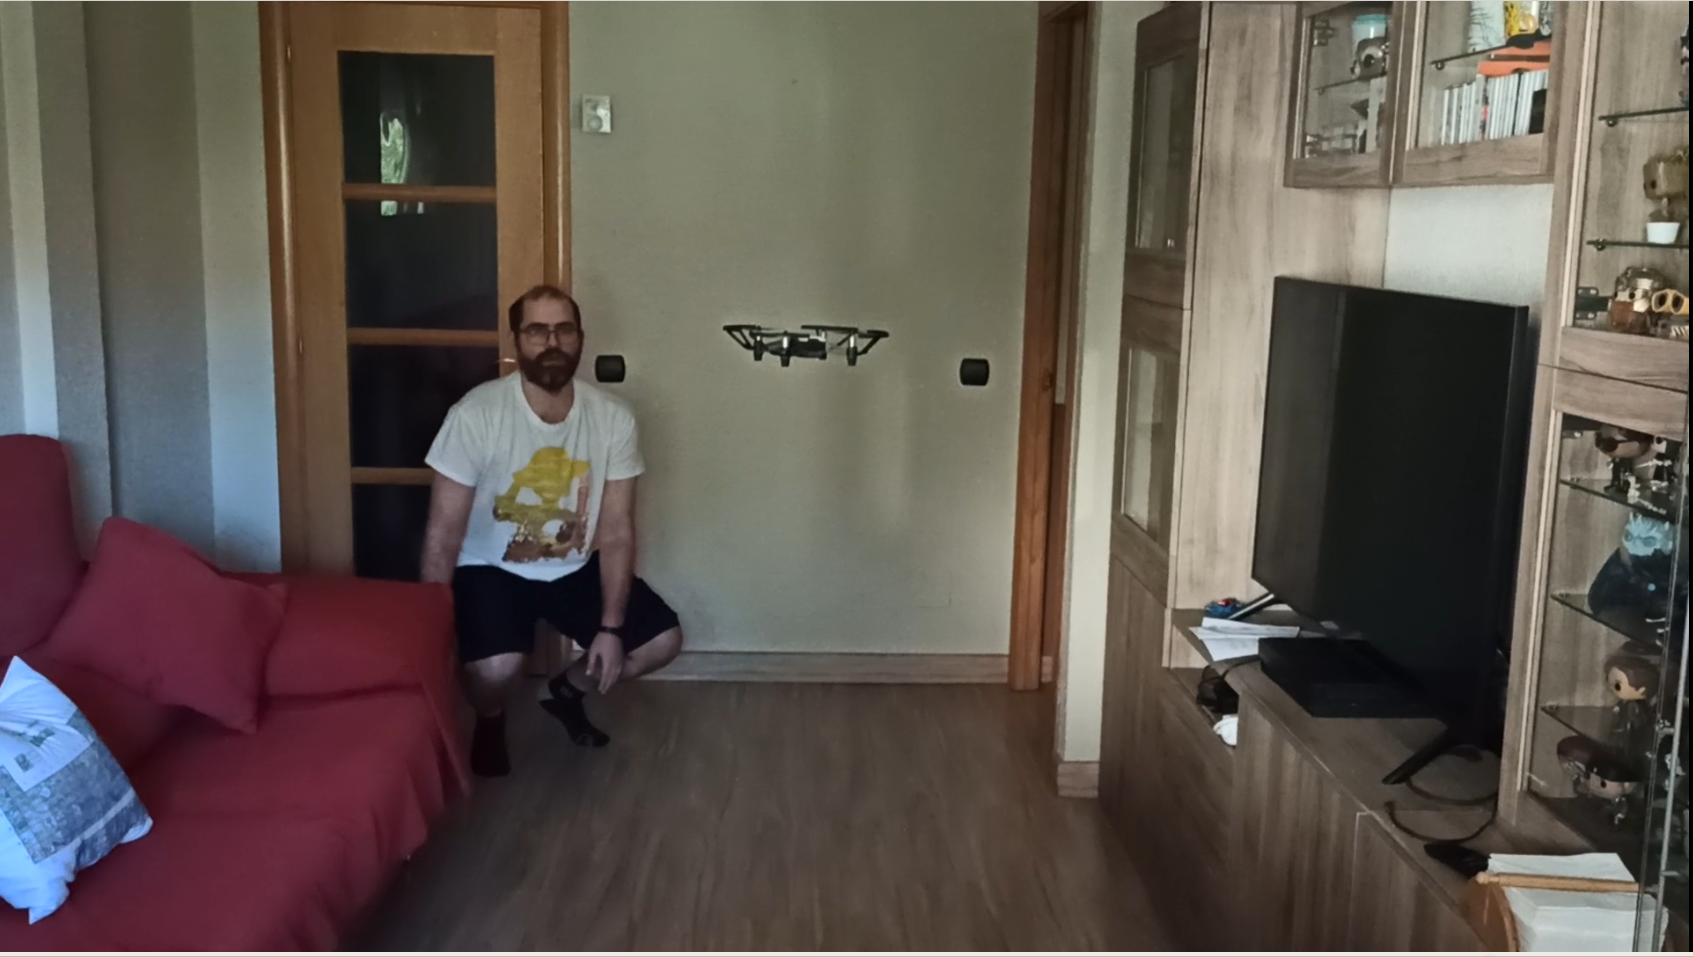
\includegraphics[width=\linewidth]{figures/real/comR_3.png}
\endminipage\hfill
\centering
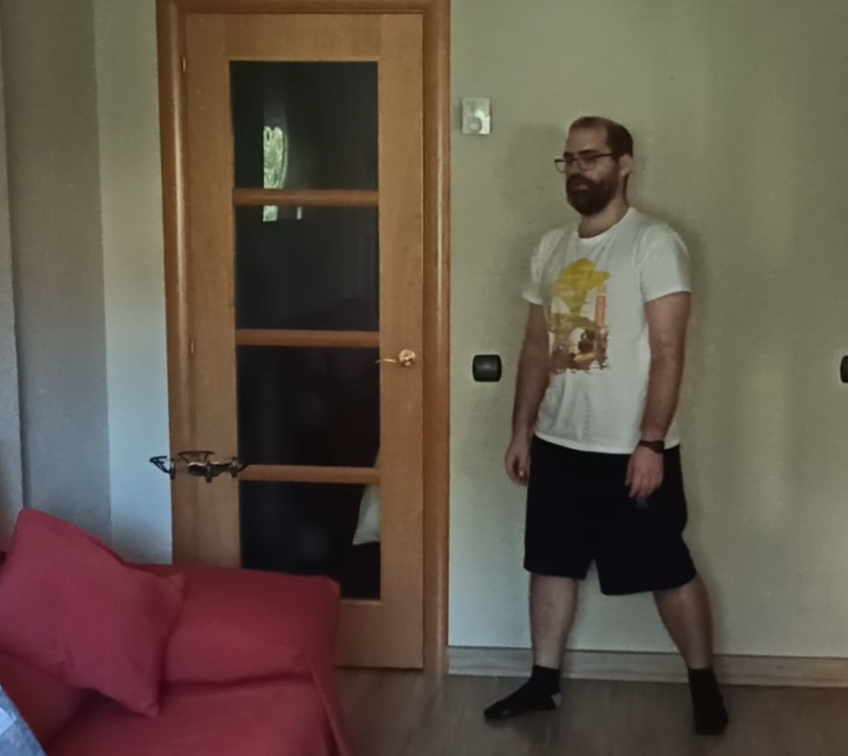
\includegraphics[width=0.45\linewidth]{figures/real/comR_2.png}\hfill
\caption{Ejemplo de ejecución típica en drone real}
\label{fig:real_com}
\end{figure}

En el vídeo se ilustra que el comportamiento deseado del drone real siguiendo a una persona que se mueve de modo natural se ha conseguido satisfactoriamente una vez ajustados los tres controladores PID.
\lhead[]{CAPÍTULO \thechapter. DRONE SIMULADO}
\chapter{Comportamiento Sigue-Persona visual con drone simulado}\label{cap.simulado}
En este capítulo se explica el software que se ha desarrollado para conseguir un comportamiento sigue persona con un drone simulado con el objetivo de ser incluido en la plataforma \textit{Kibotics} para enseñanza de robótica.

\section{Diseño}
El comportamiento en el caso simulado es casi idéntico al real, cambiando cosas propias del lenguaje en cada caso. El caso de la versión simulada es igual a la real, se compone de 2 partes claras (figura \ref{fig:esquemaReal}), la primera es la detección neuronal y la segunda los controladores PID.
\begin{figure}[H]
  \begin{center}
    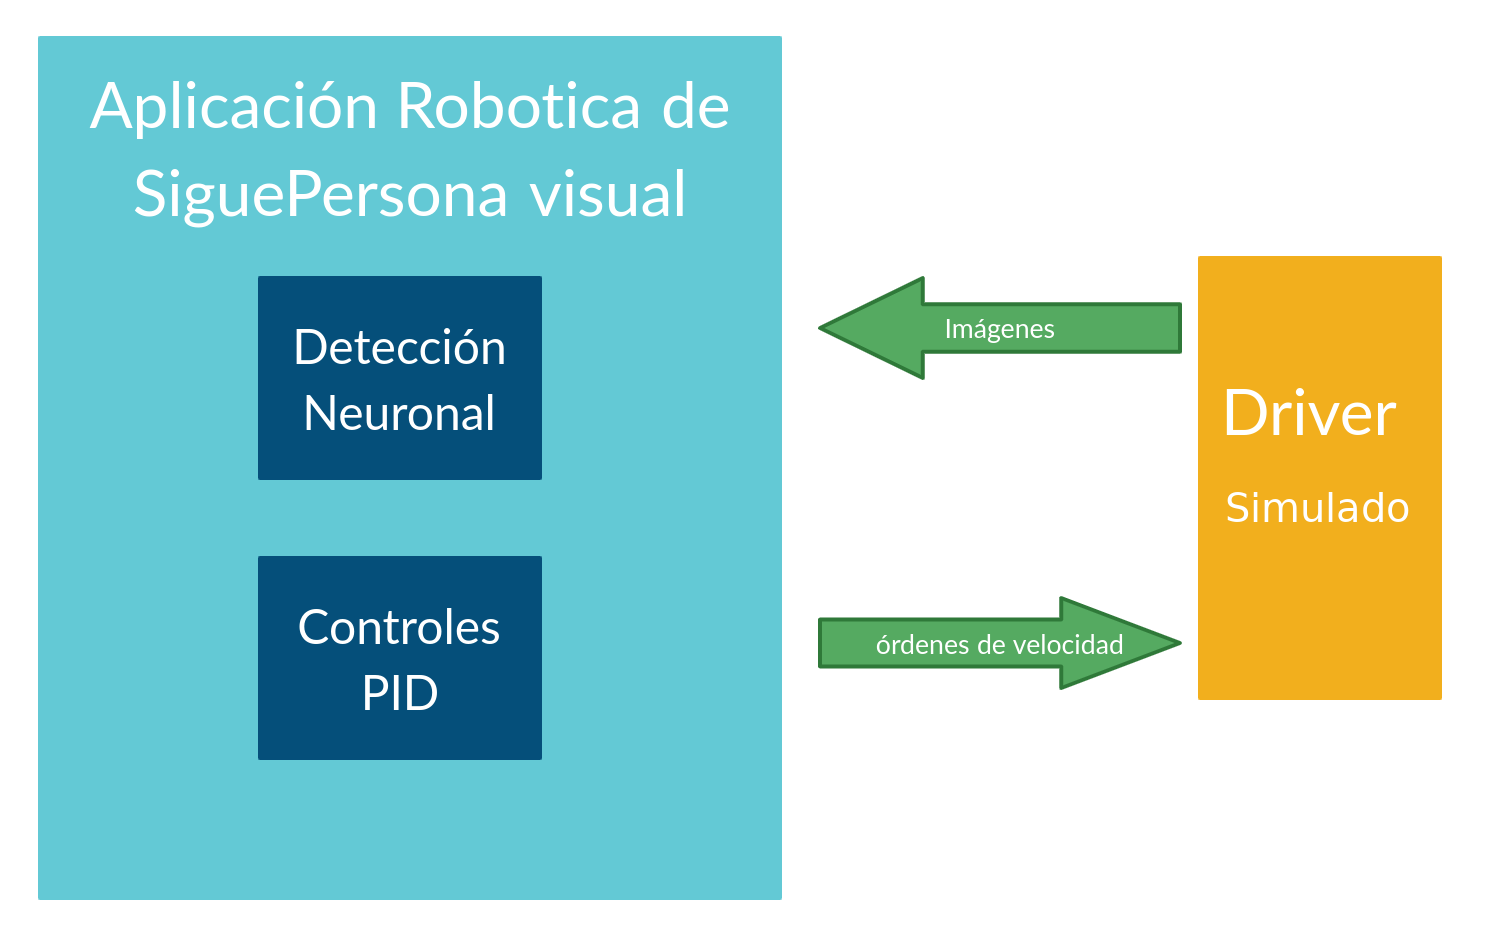
\includegraphics[width=0.7\textwidth]{figures/simulado/esquema.png}
		\caption{Diseño del comportamiento SiguePersona en su versión de simulador}
		\label{fig:esquemaSim}
		\end{center}
\end{figure}

La detección neuronal es un recubrimiento de la red neuronal que recibe las imágenes del driver y devuelve los \textit{bounding boxes}, puntuaciones y clases detectadas. 
La parte de los controladores usando los \textit{bounding boxes} calcula la velocidades y se las pasa al driver.
\section{Creación del escenario}
Lo primero es crear un escenario del simulador en el que haya un drone y una persona a la que seguir (figura \ref{fig:mundoSim}).
\begin{figure}[H]
  \begin{center}
    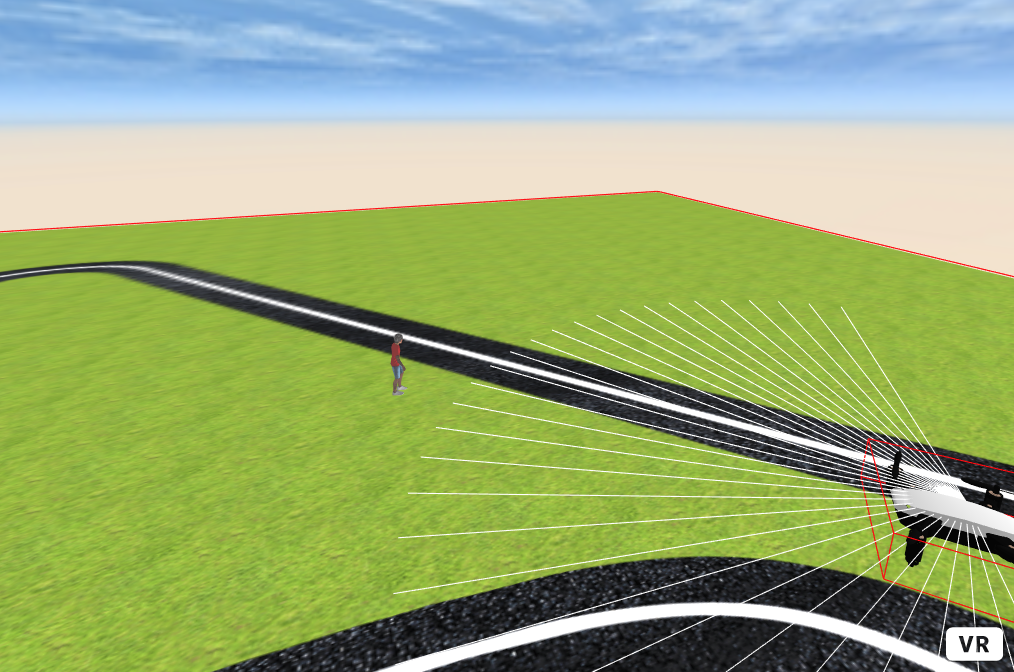
\includegraphics[width=0.7\textwidth]{figures/simulado/sim1.png}
		\caption{Mundo simulado}
		\label{fig:mundoSim}
		\end{center}
\end{figure}

Para ello se ha necesitado descargar varios modelos 3d de personas de la web mixamo \cite{mixamo} (figura \ref{fig:muneco}).
\begin{figure}[!htb]
\minipage{0.35\textwidth}
    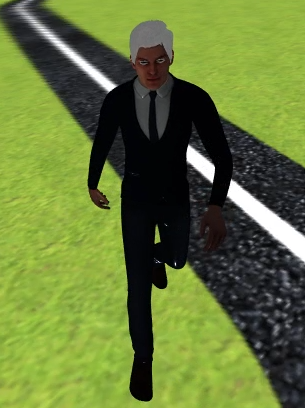
\includegraphics[width=\linewidth]{figures/simulado/muneco.png}
    \caption{Modelo 3D de persona}\label{fig:muneco}
\endminipage\hfill
\minipage{0.55\textwidth}
    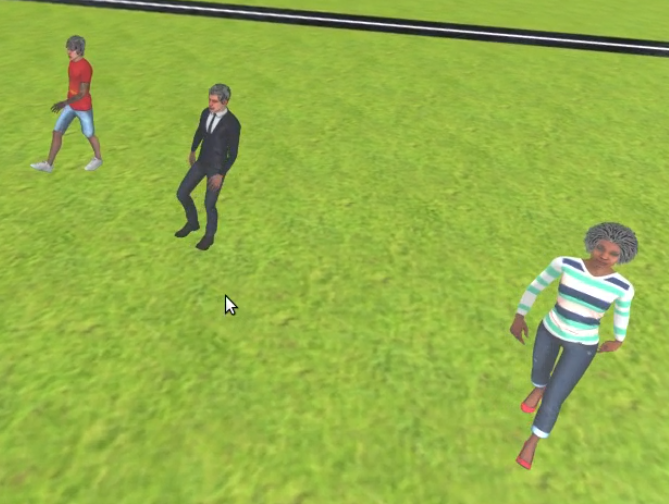
\includegraphics[width=\linewidth]{figures/simulado/persons.png}
    \caption{Modelos 3D seleccionados}\label{fig:persons}
\endminipage\hfill
\end{figure}

Los problemas que tenían estos modelos es que el simulador (\textit{websim}) los cargaba muy oscuros y con textura metálica, además de que ocupan mas de 100 MB. Para solucionar estos problemas se han cargado los modelos en \textit{Blender} para poder aclarar y quitar el metalizado de las texturas. Además se ha reducido el tamaño es estas para reducir el tamaño final de cada modelo a 3 MB.

Otro problema era que el modelo viene en un directorio con la forma de la persona en un fichero y las texturas separadas en varias imágenes. Así que se ha decidido guardarlo en un solo fichero \textit{\acrfull{glb}}. el resultado se puede ver en la figura \ref{fig:persons}.

\section{Detección visual de la persona}
Debido a las limitaciones en la capacidad de procesamiento propias del intérprete de \textit{JavaScript} en este caso no se han probado más redes y se ha optado por la que mejores resultados ha dado en tiempos de ejecución de las pruebas reales, una \textit{SSD  Mobilenet  v2} (figura \ref{fig:mobilenet}).

Se trabaja con \textit{TensorflowJS  2.0.1}. Además, se ha hecho un recubrimiento de la red para poderla usar más fácilmente permitiendo cargar la red siendo un grafo o un modelo de \textit{TensorflowJS}. También añade un postprocesado a la salida de la red.

Las red usada en \textit{Javascript} es básicamente las misma que en \textit{Python} pero con tres cambios importantes para mejorar rendimiento (figura \ref{fig:mobilenet2}):
\begin{itemize}
  \item Se elimina el postprocesado del modelo original.
  \item se suprime el \textit{NonMaxSuppression} multiclase original y se sustituye por uno de una sola clase
  \item las operaciones de \textit{NonMaxSuppression} se ejecutan en CPU para no perder tiempo en la carga de las texturas
\end{itemize}
\begin{figure}[H]
  \begin{center}
    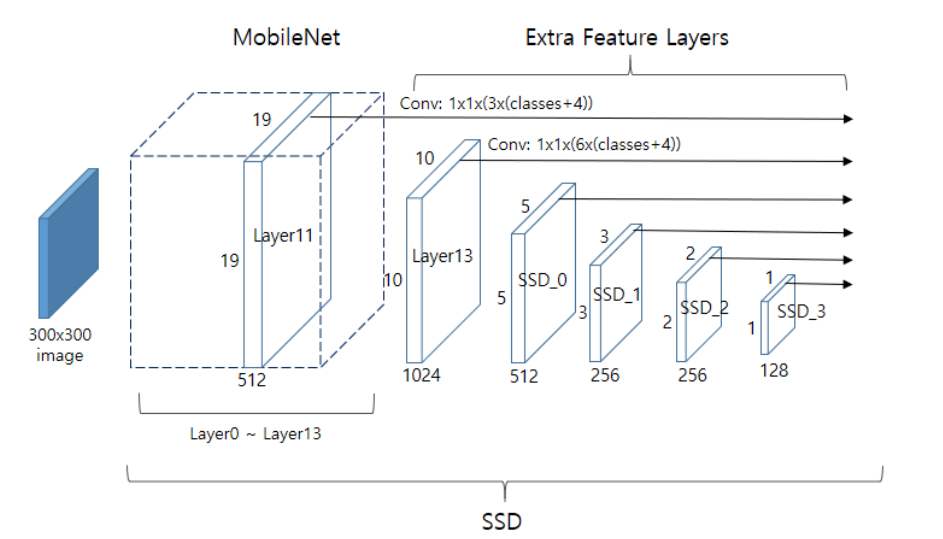
\includegraphics[width=0.8\textwidth]{figures/simulado/mobilenet.png}
		\caption{Esquema de una red Mobilenet ssd usada en \textit{TensorflowJS}}
		\label{fig:mobilenet2}
		\end{center}
\end{figure}

EL postprocesado en el caso de la versión simulada es la siguiente:
\begin{figure}[H]
  \begin{center}
    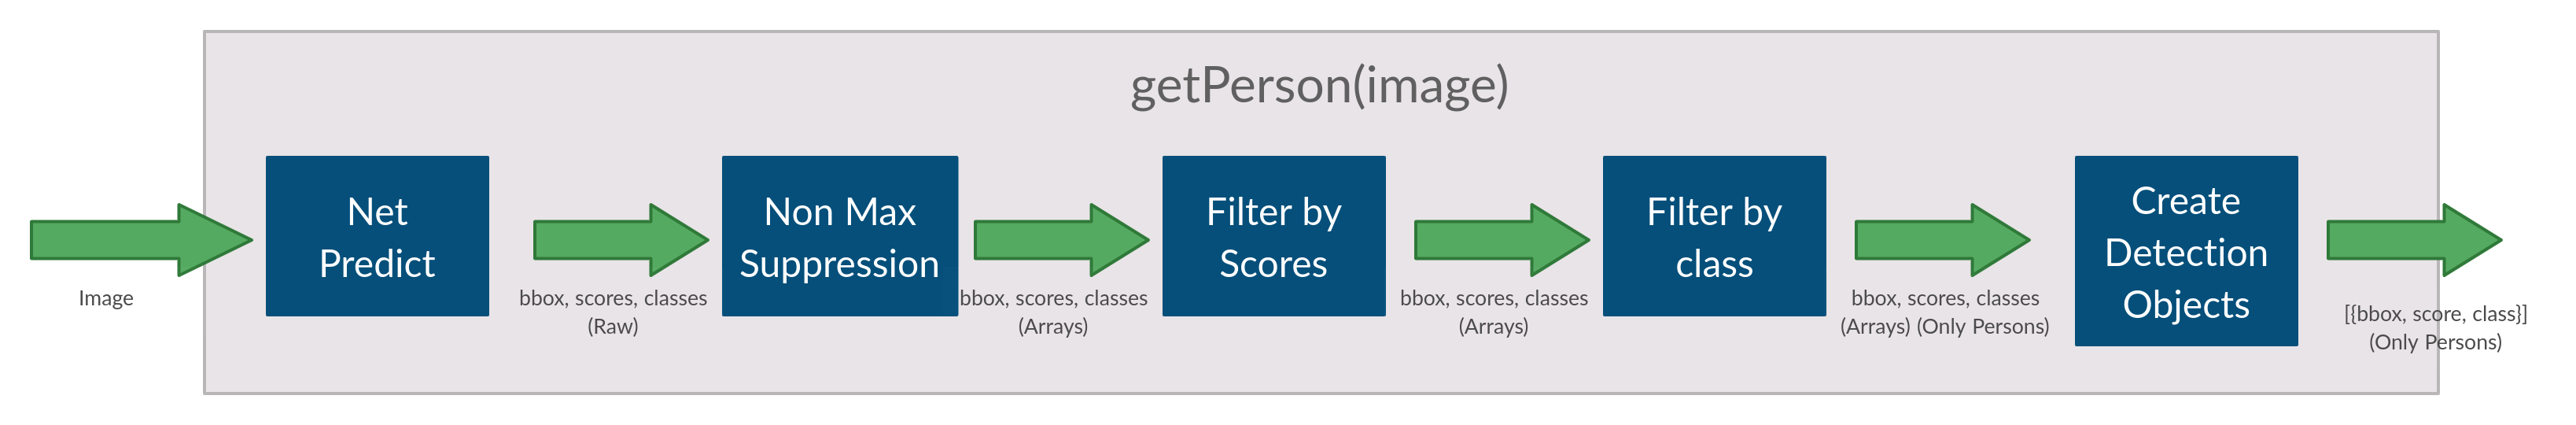
\includegraphics[width=1\textwidth]{figures/simulado/getPersonjs.png}
		\caption{Función \textit{getPerson en JS}}
		\label{fig:getPersonjs}
		\end{center}
\end{figure}
\begin{itemize}
  \item Se pasa la salida de la red por una función \textit{NonMaxSuppression} monoclase para obtener ya las detecciones, puntuaciones y clases.
  \item Se filtran detecciones para eliminar las que tengan menos que el limite indicado por configuración.
  \item Se filtra por clase para quedarnos solo con las personas.
  \item Se crea un \textit{array} de objetos que representan las detecciones (\textit{bounding box}, puntuación y clase).
\end{itemize}
Al final del postprocesado de la salida de la red se obtiene un \textit{array} con las detecciones representadas por un objeto que contiene\textbf{ \textit{bounding box}, puntuación y clase}.

Todo este procesamiento visual se ha incluido en el \textit{driver del drone simulado} para que pueda ser usado de manera sencilla desde las nuevas aplicaciones de robótica de los usuarios de \textit{Kibotics} con el simulador.

\subsection*{Creación del \textit{dataset}}
En las primeras pruebas con el drone simulado usando la red preentranada disponible en la web se observó que la detección de la persona es muy deficiente. No es capaz de detectarla en más del 50\% de los fotogramas, lo que imposibilita un seguimiento aceptable. Por lo que se decide reentrenar la red de detección con un \textit{dataset} nuevo, creado con capturas de imagen de cámara del drone \cite{github_dataset} en el simulador de \textit{Kibotics} y por ello muy adaptado a las necesidades concretas de este \acrshort{tfm}(figuras \ref{fig:dataset1} y \ref{fig:dataset2}).
\begin{figure}[!htb]
\minipage{0.45\textwidth}
    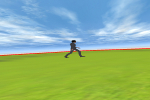
\includegraphics[width=\linewidth]{figures/simulado/person157.jpg}
    \caption{Ejemplo 1 del \textit{dataset}}\label{fig:dataset1}
\endminipage\hfill
\minipage{0.45\textwidth}
    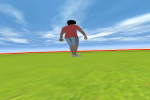
\includegraphics[width=\linewidth]{figures/simulado/person227.jpg}
    \caption{Ejemplo 2 del \textit{dataset}}\label{fig:dataset2}
\endminipage\hfill
\end{figure}

Para generar las imágenes se coloca el modelo de la persona y se va cambiando mediante código la posición del drone alrededor del modelo a 3 radios diferentes (2,5 y 10 metros) y añadiendo un nivel de aleatoriedad en el momento final del posicionado para que las imágenes no sean regulares (figura \ref{fig:esquemaCapturas}).
De esta manera se han obtenido 4000 imágenes aproximadamente. Siendo representativo de la mayoría de posiciones relativas desde las que un drone puede
tener una persona en sus cercanías. 
\begin{figure}[H]
  \begin{center}
    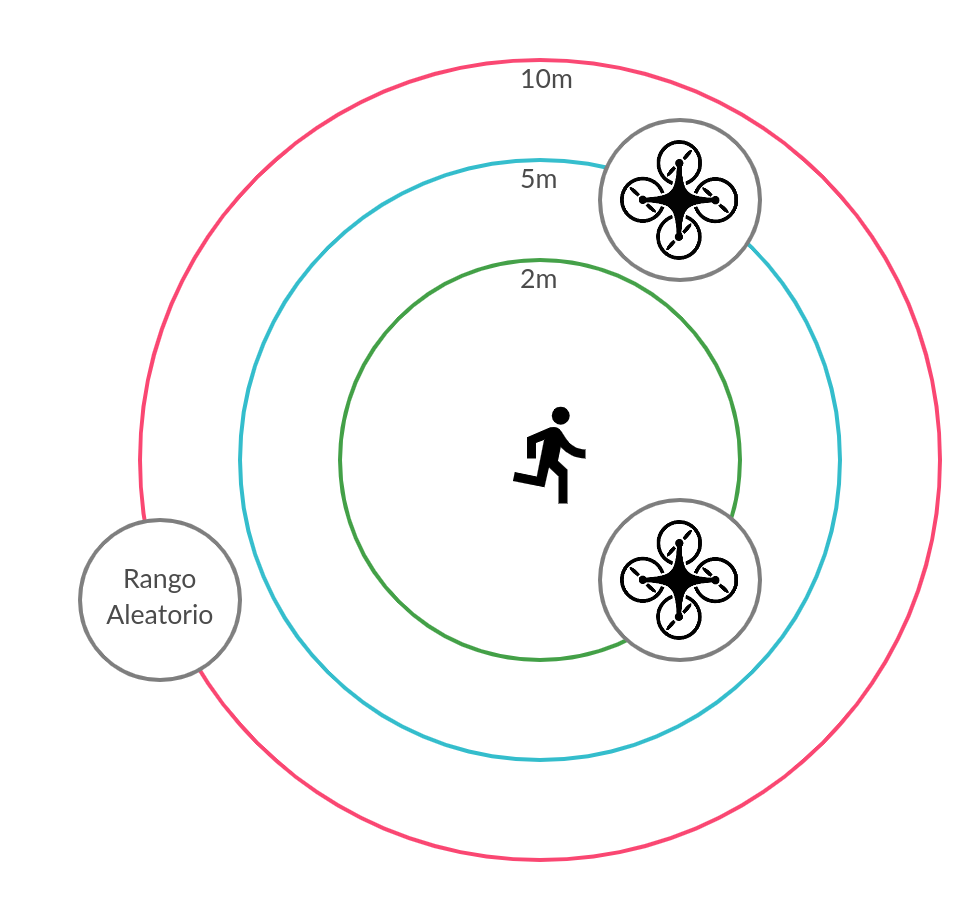
\includegraphics[width=0.6\textwidth]{figures/simulado/capturas.png}
		\caption{Posiciones relativas desde las cuales se capturan imágenes simuladas para entrenar la red de detección de personas}
		\label{fig:esquemaCapturas}
		\end{center}
\end{figure}
Una vez generadas todas las capturas se han etiquetado manualmente, para ello se han subido a la web \textit{LabelMe}, que permite etiquetar las imágenes (Figura \ref{fig:datasetlabelme}).
\begin{figure}[H]
  \begin{center}
    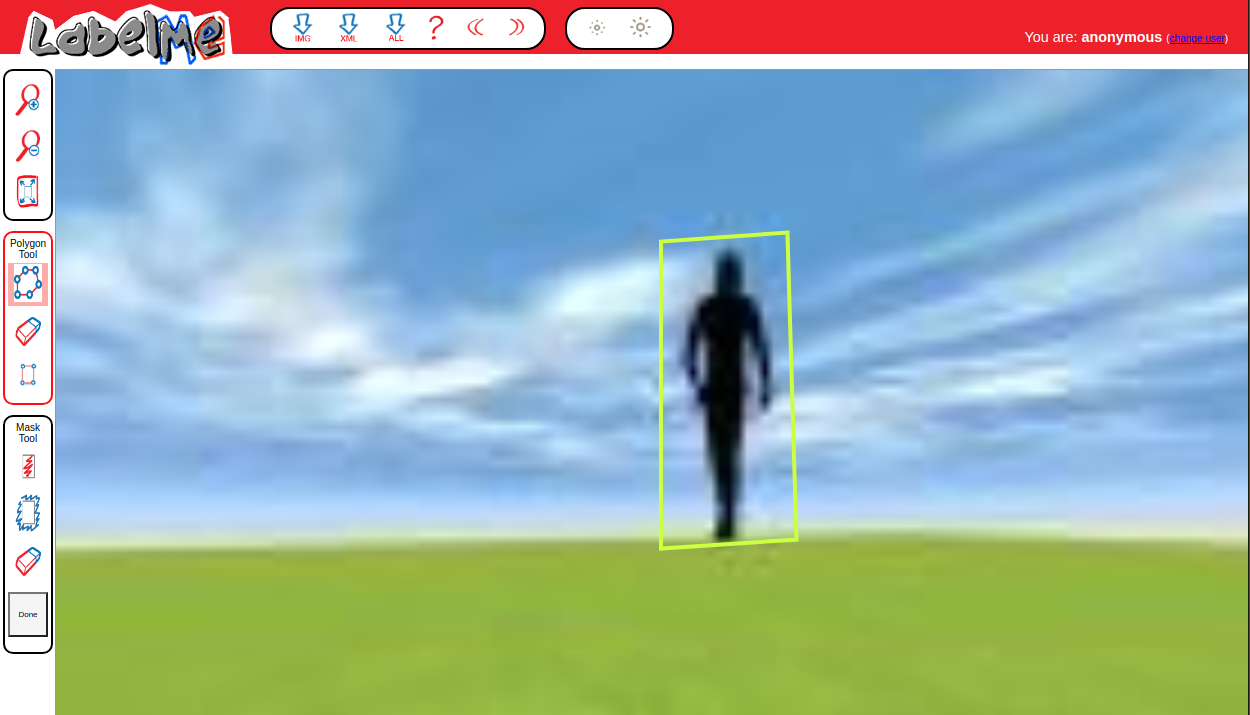
\includegraphics[width=0.6\textwidth]{figures/herramientas/labelme.png}
		\caption{Etiquetado del \textit{dataset} en  \textit{LabelMe}}
		\label{fig:datasetlabelme}
		\end{center}
\end{figure}
Cuando están todas etiquetadas, se descargan, Son un conjunto de imágenes y ficheros \textit{XML}.

Para aumentar el tamaño del dataset se ha seguido una técnica de "data augmentation", con idea que el entrenamiento de la red neuronal sea más rico. Se ha procedido  a espejar las imágenes ya etiquetadas mediante un \textit{script} de \textit{python}, doblando el tamaño de \textit{dataset}. Después de esto se ha dividido en \textit{train} y \textit{test}, dejando un 10\% para la segunda parte mediante otro \textit{script}.

Los dos últimos pasos han sido convertir esos ficheros \textit{XML} en uno \textit{CSV} para \textit{train} y otro para \textit{test} para poder manejar mejor el \textit{dataset} y crear ficheros \textit{record} (ficheros binarios que contienen tanto imágenes como anotaciones) para poderlos usar mejor en los entrenamientos de \textit{Tensorflow}.
\subsection*{Reentrenar red}
El reentrenamiento se ha efectuado en \textbf{Google Colab} mediante un cuadernillo \textit{Python}. La primera intención fue hacerse con \textit{Tensorflow 2.0} pero \textit{Object Detection API} todavía no tiene soporte para guardar las redes entrenadas en formato grafo, por lo que no ha podido usarse en el navegador al tener unos tiempos de detección superiores al segundo.

Para subsanar este contratiempo se ha desarrollado uno equivalente para \textit{Tensorflow 1.15}, donde sí hay soporte para grafos. Dicho entrenamiento ha consistido en 20.000 iteraciones con un \textit{batch} de 24 imágenes.
se han obtenido los siguientes resultados: 
\begin{table}[H]
\centering
\begin{tabular}{|c|c|}

\multicolumn{2}{c}{\textbf{Resultados}} \\ \hline
Precision             & 0.64            \\ \hline
Recall                & 0.69            \\ \hline
\end{tabular}
\caption{Resultados del entrenamiento}
\label{tab:cambios_python_2_3}
\end{table}

Además se han obtenido una pérdida del 0.3. Con estos datos junto con una pequeña bajada del limite de confianza se ha conseguido que la detección en el simulador ronde el 80\%. De esta manera ya es posible seguir la persona sin problemas en el simulador que ejecuta en el navegador.

\section{controles PID}
Una vez que se procesa la imagen recibida de el drone y se tienen las detecciones de personas, se selecciona la persona con mayor puntuación y de su \textit{bounding box} se extrae posición central y el área. En este caso no se hace control vertical porque las imágenes recibidas no permiten un control aceptable en este eje.
\begin{figure}[H]
  \begin{center}
    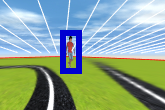
\includegraphics[width=0.7\textwidth]{figures/simulado/sim3.png}
		\caption{función \textit{Detección ideal}}
		\label{fig:sim3}
		\end{center}
\end{figure}

Para controlar el drone se va a hacer con dos velocidades, avance horizontal y giro horizontal. Para ello se utiliza un control PID (en este caso debido al funcionamiento del drone solo proporcional y derivativo) para cada una de las velocidades.

\subsection*{Control de avance horizontal}

En el caso de la velocidad de avance, se toma como referencia el área. Se fija un área objetivo para el \textit{bounding box}, si la obtenida es menor se avanza y si es mayor se retrocede. Las constantes \textbf{proporcional y derivativa} en este caso son \textbf{0.01 y 0} respectivamente. Los valores de las constantes son diferentes porque dependen del comportamiento del robot en cuestión, incluso en robots del mismo modelo pueden variar estos valores ligeramente.

\subsection*{Control de giro horizontal o guiñada}

En este caso se toma como referencia la coordenada x del centro de la imagen. Si el \textit{bounding box} se mueve a la izquierda hay que girar a la izquierda y si se va a derecha igual. Las constantes \textbf{proporcional y derivativa} en este caso son \textbf{0.002 y 0.0001} respectivamente.

\section{Validación experimental}
La validación experimental del desarrollo se ha hecho en 3 casos: un test unitario por cada \textit{PID}  un test global del conjunto. En todos los casos el bucle de control funciona a 7 \acrshort{fps}.

\subsection{Control de giro horizontal}
Esta prueba consiste en colocar uno de los modelos 3D moviéndose de izquierda a derecha delante del drone, mediante una animación de A-frame\footnote{\url{https://aframe.io}}. Permite ajustar las constantes del \textit{PID} de giro horizontal\footnote{\url{https://www.youtube.com/watch?v=xLa3wSYIIuY}} (figura \ref{fig:sim_giro}).

\begin{figure}[!htb]
\minipage{0.3\textwidth}
    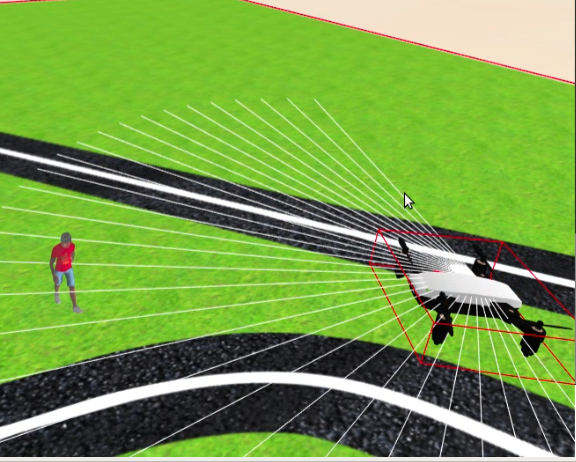
\includegraphics[width=\linewidth]{figures/simulado/giro_1.png}
\endminipage\hfill
\minipage{0.3\textwidth}
    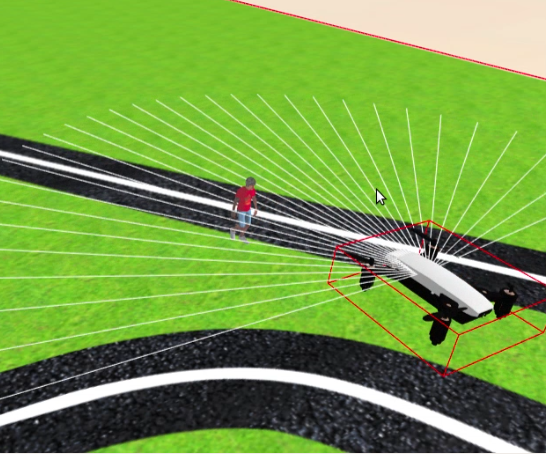
\includegraphics[width=\linewidth]{figures/simulado/giro_2.png}
\endminipage\hfill
\minipage{0.3\textwidth}
    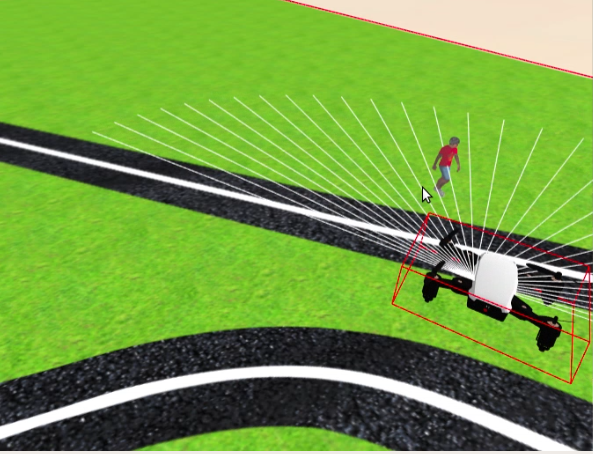
\includegraphics[width=\linewidth]{figures/simulado/giro_3.png}
\endminipage\hfill
\caption{Ejemplo de giro horizontal}
\label{fig:sim_giro}
\end{figure}
\subsection{Control de avance}
Esta prueba consiste en colocar uno de los modelos 3D de persona alejándose y acercándose al drone para ajustar las constantes del \textit{PID} de avance\footnote{\url{https://www.youtube.com/watch?v=CNo6rionlcE}} (figura \ref{fig:sim_avance}).

\begin{figure}[!htb]
\minipage{0.3\textwidth}
    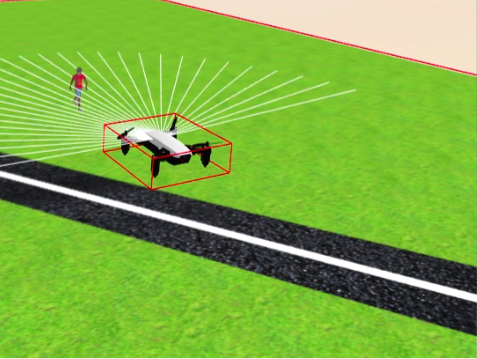
\includegraphics[width=\linewidth]{figures/simulado/avance_1.png}
\endminipage\hfill
\minipage{0.3\textwidth}
    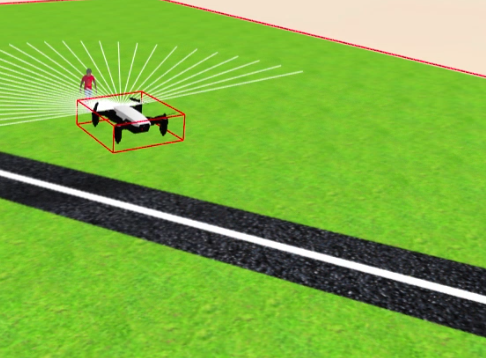
\includegraphics[width=\linewidth]{figures/simulado/avance_2.png}
\endminipage\hfill
\minipage{0.3\textwidth}
    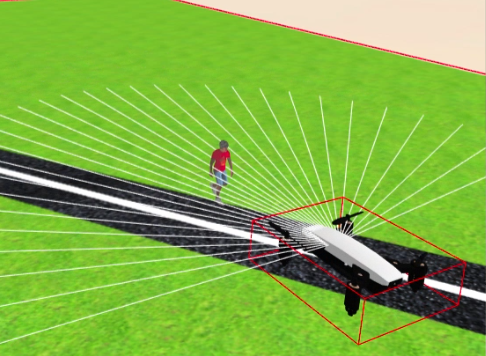
\includegraphics[width=\linewidth]{figures/simulado/avance_3.png}
\endminipage\hfill
\caption{Ejemplo de avance}
\label{fig:sim_avance}
\end{figure}
\subsection{Ejecución típica completa}
En este caso en vez de usar una animación, se le ha conectado un teleoperador existente en \textit{Websim}, que permite controlar un objeto en el mundo simulado con las flechas del teclado, para poder mover libremente el modelo 3D de la persona para que lo siga el \textit{drone} (figura \ref{fig:ejecucion_sim}). Si el movimiento no es el esperado, toca ajustar las constantes oportunas.

% \begin{figure}[H]
%   \begin{center}
%   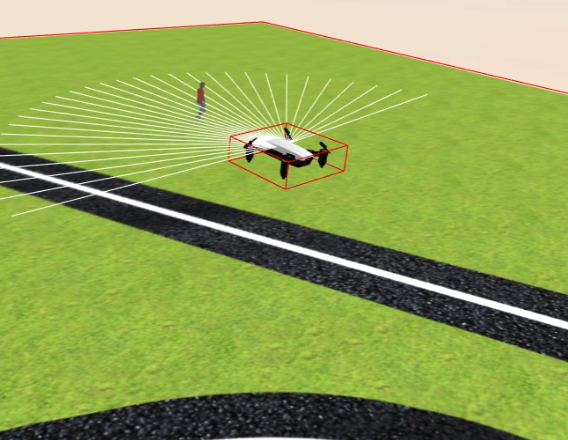
\includegraphics[width=0.7\textwidth]{figures/simulado/comp_1.png}\hfill
%   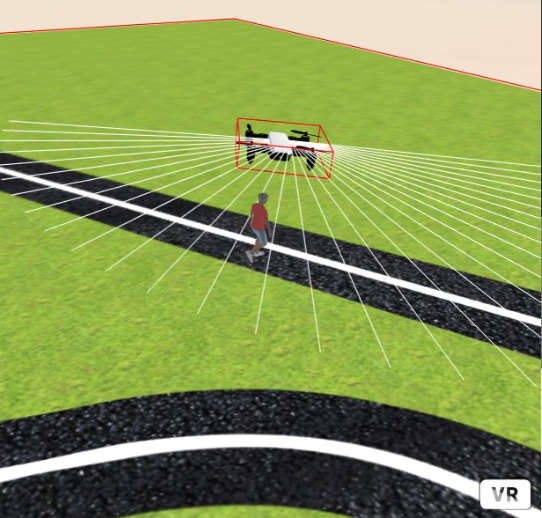
\includegraphics[width=0.7\textwidth]{figures/simulado/comp_2.png}\hfill
%     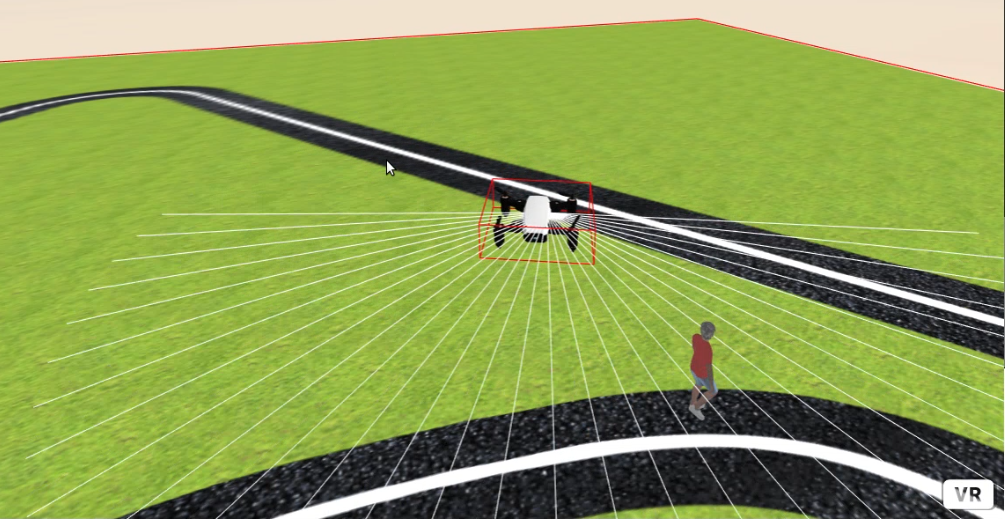
\includegraphics[width=0.7\textwidth]{figures/simulado/comp_3.png}\hfill
% 		\caption{Ejecución Típica}
% 		\label{fig:ejecucion_sim}
% 		\end{center}
% \end{figure}

\begin{figure}[!htb]
\minipage{0.3\textwidth}
    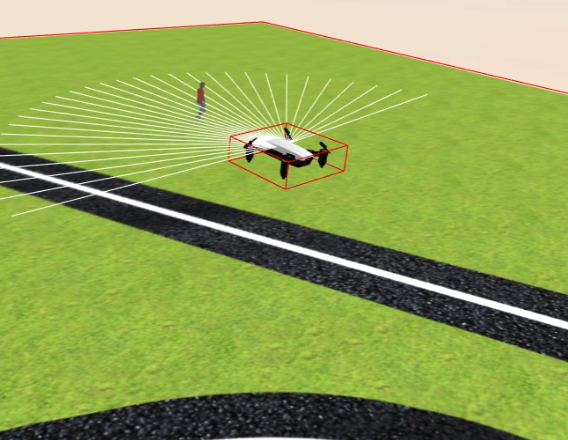
\includegraphics[width=\linewidth]{figures/simulado/comp_1.png}
\endminipage\hfill
\minipage{0.3\textwidth}
    \includegraphics[width=\linewidth]{figures/simulado/comp_2.png}
\endminipage\hfill
\minipage{0.3\textwidth}
    \includegraphics[width=\linewidth]{figures/simulado/comp_3.png}
\endminipage\hfill
\caption{Ejecución Típica}
\label{fig:ejecucion_sim}
\end{figure}



\lhead[]{CAPÍTULO \thechapter. CONCLUSIONES}
\chapter{Conclusiones}\label{cap.conclusiones}
Una vez documentado el software diseñado y desarrollado a lo largo de este \acrshort{tfm} y la funcionalidad que ofrece, se dedica este capítulo a la comprobación de los objetivos alcanzados, así como a la explicación de los conocimientos adquiridos y una breve exposición de posibles mejoras y de las líneas de actuación futuras.
\section{Conclusiones}
El objetivo principal, que era la creación de la infraestructura necesaria para añadir procesamiento visual complejo, de manera sencilla de usar, se ha cumplido, ahora ya se pueden desarrollar prácticas tanto con drone simulado como real de detección robusta de personas.
\newline

En cuanto a los subobjetivos concretos, se ha conseguido un comportamiento robótico \textit{siguePersona} visual real gracias al uso de \textit{Tensorflow} y \textit{Opencv} para detectar a la persona y el uso de varios controladores PID para las velocidades. Para lograr este subobjetivo se han creado clases de \textit{Python} para contener las las redes y permitir un nivel de abstracción mayor además de simplificar su uso mediante métodos personalizados como \textit{getPerson() en \textit{Python}}. Igualmente se ha mejorado el driver de Python del drone real DJI Tello, que permite control en velocidad y un envío más rápido y fiable de comandos desde el ordenador al propio drone volador.
\newline

También se ha cumplido el subobjetivo del comportamiento \textit{siguePersona} visual simulado, teniendo que crear un mundo que se adaptara a la necesidades y creando clases de \textit{Javascript} para contener las las redes y permitir un nivel de abstracción mayor además de para simplificar su uso mediante el método \textit{getPerson} en \textit{JavaScript}. Además, para este subobjetivo se ha necesitado crear un \textit{dataset} específico de 4000 imágenes y reentrenar una red de detección visual puesto que la red preentrenada disponible no funcionaba satisfactoriamente. Se ha utilizado TensorlfowJS de modo que la inferencia neuronal ejecuta en el navegador web en tiempo real.
\newline

De manera personal, también se ha alcanzado el objetivo de mejorar en conocimientos en el campo del desarrollo web y el modelado 3D. Gracias a ello se han adquirido conocimientos en tecnologías web de procesado de imagen como \textit{OpenCVJS} y \textit{TensorflowJS }que en un principio creía que era inviable por la necesidad de recursos que tiene y las limitaciones propias del intérprete de \textit{JavasScript}.
\section{Trabajos futuros}
Las contribuciones de este \acrshort{tfm} han abierto las posibilidades para desarrollar nuevas prácticas utilizando visión de manera sencilla de la plataforma \textit{Kibotics} manteniendo la reobusted habitual de las redes neuronales. Pero esto es solo el principio, algunas mejoras pueden ser:

\begin{itemize}
  \item \textbf{Creación de prácticas que utilicen esta tecnología}. Se ha asentado la base, pero ahora toca desarrollar nuevas prácticas de seguimiento de personas o de otros objetos como señales de tráfico, semáforos, etc.
  \item \textbf{Aumentar el número de opciones en cuanto a detección}, como por ejemplo un sigue persona que detecte caras para poder seguir a una persona concreta en un grupo
\end{itemize}


%%%%%%%%%%%%%%% Bibliograí­a %%%%%%%%%%%%%%%
\nocite{*}
\bibliographystyle{unsrt}
\bibliography{Bibliografia.bib}
\addcontentsline{toc}{chapter}{Bibliografía}

\end{document}
